\documentclass[14pt]{beamer}
%\documentclass[handout]{beamer} %Makes Handouts
\usetheme{Singapore} %Gray with fade at top
\useoutertheme[subsection=false]{miniframes} %Supppress subsection in header
\useinnertheme{rectangles} %Itemize/Enumerate boxes
\usecolortheme{seagull} %Color theme
\usecolortheme{rose} %Inner color theme

\definecolor{light-gray}{gray}{0.75}
\definecolor{dark-gray}{gray}{0.55}
\setbeamercolor{item}{fg=light-gray}
\setbeamercolor{enumerate item}{fg=dark-gray}

\setbeamertemplate{navigation symbols}{}
%\setbeamertemplate{mini frames}[default]
%\setbeamercovered{dynamics}
\setbeamerfont*{title}{size=\Large,series=\bfseries}

%\setbeameroption{notes on second screen} %Dual-Screen Notes
%\setbeameroption{show only notes} %Notes Output

\setbeamertemplate{frametitle}{\vspace{.5em}\bfseries\insertframetitle}
\newcommand{\heading}[1]{\noindent \textbf{#1}\\ \vspace{1em}}

% small footnotes
\setbeamerfont{footnote}{size=\tiny}

\usepackage{bbding,color,multirow,times,ccaption,tabularx,graphicx,verbatim,booktabs,fixltx2e}
\usepackage{colortbl} %Table overlays
\usepackage[english]{babel}
\usepackage[latin1]{inputenc}
\usepackage[T1]{fontenc}
\usepackage{lmodern}
\usepackage{alltt}

\author[]{Thomas J. Leeper}
\institute[]{
  \inst{}%
  Department of Political Science and Government\\Aarhus University
}

\usepackage{tikz}
\usetikzlibrary{shapes,arrows}
\usepackage[normalem]{ulem}

\title{Running Online Surveys with Nonprobability Samples}

\date[]{10 December 2015\\EUI Quantitative Methods Working Group}

\begin{document}

\frame{\titlepage}

\frame{
\frametitle{Overview}
\begin{itemize}\itemsep1em
\item What is this course about?
\item Who are you?
\end{itemize}
}


\frame{
\frametitle{Learning Goals}

By the end of today you should be able to:

\begin{itemize}\itemsep1em
\item Describe logic of design-based and model-based representativeness
\item Evaluate the quality of a convenience sample
\item Design simple web forms using several tools
\item Evaluate trade-offs between various technologies for behavioral research
\item Apply all of this to your own research
\end{itemize}
}

\frame{\tableofcontents}


\frame{
\frametitle{Introductions}

\begin{itemize}\itemsep1em
\item Who are you?
\item What field are you from?
\end{itemize}
}

\frame{
\frametitle{About Me}

\begin{itemize}\itemsep1em
\item Assistant Professor at London School of Economics since September
\item Postdoc at Aarhus University 2012--2015
\item PhD in Political Science from Northwestern University (2015)
\item Interested in:
	\begin{itemize}
	\item Political psychology
	\item Survey--experimental methods
	\item Reproducible computational social science
	\end{itemize}
\end{itemize}
}

\bgroup
\setbeamercolor{background canvas}{bg=blue!20!white}
\setbeamertemplate{navigation symbols}{}
\begin{frame}[plain]{}
\frametitle{How many of you have\dots}

\begin{itemize}\itemsep1em
\item<2-> taken a course on survey methods?
\item<3-> taken a course on experimental design?
\item<4-> written HTML markup before?
\item<5-> run a study on MTurk or Crowdflower, with a vendor like YouGov, or another online platform?
\end{itemize}
\end{frame}
\egroup

\section{``The Gold Standard''}
\frame{\tableofcontents[currentsection]}


\frame{
\frametitle{``The Gold Standard''}

\begin{quote}\small
a population-based experiment uses survey sampling methods to produce a collection of experimental subjects that is representative of the target population of interest for a particular theory \dots the population represented by the sample should be representative of the population ot which the researcher intends to extend his or her findings. In population-based experiments, experimental subjects are randomly assigned to conditions by the researcher
\end{quote}

{\footnotesize p2. from Mutz, Diana. 2011. \textit{Popuation-Based Survey Experiments}. Princeton University Press.\par}

}

% design-based experimental inference
\frame{
	\frametitle{Causal Inference in Experiments I}
	\begin{itemize}\itemsep0.5em
    	\item<1-> Causal inference is a comparison of two \textit{potential outcomes}
    	\item<2-> A potential outcome is the value of the outcome (Y) for a given unit (i) after receiving a particular version of the treatment (X)
    	\item<3-> Each unit has multiple \textit{potential} outcomes, but we only observe one of them
    	\item<4-> A \textit{causal effect} is the difference between these (e.g., $Y_{X=1} - Y_{X=0}$), all else constant
	\end{itemize}
}

\frame{
	\frametitle{Causal Inference in Experiments II}
	\begin{itemize}\itemsep2em
    	\item<1-> We cannot see individual-level causal effects
    	\item<2-> We can see \textit{average causal effects}
    		\begin{itemize}
        		\item<2-> Ex.: Average difference in participation between those with and without university degrees
    		\end{itemize}
    	\item<3-> We want to know: $TE_i = Y_{1i} - Y_{0i}$
	\end{itemize}
}

\frame{
	\frametitle{Causal Inference in Experiments III}
	\begin{itemize}\itemsep1em
		\item<1-> We want to know: $TE_i = Y_{1i} - Y_{0i}$
		\item<2-> We can average: $ATE = E[Y_{1i} - Y_{0i}] = E[Y_{1i}] - E[Y_{0i}]$
		\item<3-> But we still only see one potential outcome for each unit:\\ \vspace{1em}
    		$ATE_{naive} = E[Y_{1i} | X = 1] - E[Y_{0i} | X = 0]$
    	\item<4-> Is this what we want to know?
	\end{itemize}
}


\frame{
	\frametitle{Causal Inference in Experiments IV}
	\begin{itemize}\itemsep1em
	\item What we want and what we have:
		\begin{align}
		ATE & = E[Y_{1i}] - E[Y_{0i}] \\[1em]
		ATE_{naive} & = E[Y_{1i} | X = 1] - E[Y_{0i} | X = 0]
		\end{align}		
	\item<2-> Are the following statements true?\\
  		\begin{itemize}\itemsep1em
      		\item<2-> $E[Y_{1i}] = E[Y_{1i} | X = 1]$
      		\item<2-> $E[Y_{0i}] = E[Y_{0i} | X = 0]$
  		\end{itemize}
  	\item<3-> Not in general!
  	\end{itemize}
}

\frame{
	\frametitle{Causal Inference in Experiments V}
	\begin{itemize}\itemsep1em
    	\item Only true when both of the following hold:
    	\begin{align}
    	E[Y_{1i}] = E[Y_{1i} | X = 1] = E[Y_{1i} | X = 0]\\
    	E[Y_{0i}] = E[Y_{0i} | X = 1] = E[Y_{0i} | X = 0]
    	\end{align}
    	\item In that case, potential outcomes are \textit{independent} of treatment assignment
		\item If true, then:
    	\begin{align*}
    	ATE_{naive} & = E[Y_{1i} | X = 1] - E[Y_{0i} | X = 0] \tag{5}\\
    	& = E[Y_{1i}] - E[Y_{0i}]\\
    	& = ATE
    	\end{align*}
	\end{itemize}
}

\frame{
	\frametitle{Causal Inference in Experiments VI}
	\begin{itemize}\itemsep0.5em
    	\item This holds in experiments because of randomization\\
    		\begin{itemize}
        		\item Units differ only in what side of coin was up
        		\item Experiments randomly reveal potential outcomes
    		\end{itemize}
    	\item<2-> Matching/regression/etc. attempts to eliminate those confounds, such that:
    	\begin{align*}
    	E[Y_{1i} | Z] = E[Y_{1i} | X = 1, Z] = E[Y_{1i} | X = 0, Z]\\
    	E[Y_{0i} | Z] = E[Y_{0i} | X = 1, Z] = E[Y_{0i} | X = 0, Z]
    	\end{align*}
	\end{itemize}
}

\frame{}


% design-based survey sampling

\frame{
	\frametitle{Surveys Start with an Inference Population}
	\begin{itemize}\itemsep1em
		\item We want to speak to a population
		\item But what population is it?
			\begin{itemize}
			\item<2-> A national population?
			\item<3-> Adults in Western, industrialized democracies?
			\item<4-> All human beings?
			\end{itemize}
		\item<5-> This is rarely specified, but is important when we think about whether a sample is appropriate
	\end{itemize}
}


\bgroup
\setbeamercolor{background canvas}{bg=blue!20!white}
\setbeamertemplate{navigation symbols}{}
\begin{frame}[plain]{}
\frametitle{Think about your own work}


\vspace{1em}

Consider the following: 

\begin{enumerate}\itemsep1em
\item What is your research about?
\item What population do you aim to generalize to?
\end{enumerate}

\vspace{1em}

Discuss with the person next to you.
\end{frame}
\egroup






\frame{
	\frametitle{A Hypothetical Census}

	\begin{itemize}\itemsep2em
		\item Advantages
			\begin{itemize}
				\item<2-> Perfectly representative
				\item<2-> Sample statistics are population parameters
			\end{itemize}
		\item Disadvantages
			\begin{itemize}
				\item<3-> Costs
				\item<3-> Feasibility
				\item<3-> Need
			\end{itemize}		
	\end{itemize}
}


\frame{\frametitle{So, instead we sample!}}


\frame{
	\frametitle{Sampling Frames}
	\begin{itemize}\itemsep1em
		\item Enumeration (listing) of all units eligible for sample selection
		\item Random sample from that list
		\item<2-> Building a sampling frame
			\begin{itemize}
			\item Combine existing lists
			\item Canvass/enumerate from scratch
			\end{itemize}
		\item<3-> Concern about coverage: Does frame match population?
	\end{itemize}
}


\frame{
	\frametitle{Sample Estimates from an SRS}
	\begin{itemize}\itemsep1em
		\item Each unit in frame has equal probability of selection
		\item Sample statistics are unweighted
		\item Variances are easy to calculate
		\item Easy to calculate sample size need for a particular variance
	\end{itemize}
}

\frame{
	\frametitle{Sample mean}
	\begin{equation}
	\bar{y} = \frac{1}{n}\sum_{i=1}^{n}y_i
	\end{equation}
	where $y_i = $ value for a unit, and\\
	$n = $ sample size
	
	\begin{equation}
	SE_{\bar{y}} = \sqrt{(1-f)\frac{s^2}{n}}
	\end{equation}
	where $f = $ proportion of population sampled,\\
	$s^2 = $ sample element variance, and\\
	$n = $ sample size
}

\frame{
	\frametitle{Estimating sample size}

\small

	If all we cared about was a single proportion:

	\begin{equation}
		Var(p) = (1-f)\frac{p(1-p)}{n-1}
	\end{equation}
	
	Given a large population:	
	\begin{equation}
		Var(p) = \frac{p(1-p)}{n-1}
	\end{equation}
	
	Need to solve the above for $n$.
	\begin{equation}
	\only<2->{n = \frac{p(1-p)}{v(p)} = \frac{p(1-p)}{SE^2}}
	\end{equation}
}

\frame{
	\frametitle{Estimating sample size}
    Determining sample size requires:
    	\begin{itemize}
    		\item A possible value of $p$
    		\item A desired precision (standard error)
    	\end{itemize}
	\vspace{1em}
	If support for each coalition is evenly matched ($p = 0.5$):
	\begin{equation}
	n = \frac{0.5(1-0.5)}{SE^2} = \frac{0.25}{SE^2}
	\end{equation}
}

\frame{
	\frametitle{Estimating sample size}
	What precision (margin of error) do we want?
	\begin{itemize}
		\item +/- 2 percentage points: $SE = 0.01$
			\begin{equation}
			n = \frac{0.25}{0.01^2} = \frac{0.25}{0.0001} = 2500
			\end{equation}
		\item<2-> +/- 5 percentage points: $SE = 0.025$
			\begin{equation}
			n = \frac{0.25}{0.000625} = 400
			\end{equation}
		\item<3-> +/- 0.5 percentage points: $SE = 0.0025$
			\begin{equation}
			n = \frac{0.25}{0.00000625} = 40,000
			\end{equation}
	\end{itemize}
}



\frame{

\frametitle{Sampling Considerations\dots}

\begin{itemize}\itemsep1em
\item<2-> More complex designs possible, all based on each unit having a \textit{known, non-zero} probability of being sampled
	\begin{itemize}
	\item Stratified sampling can produce lower variances
	\end{itemize}
\item<3-> Random sampling ensures that samples are, \textit{in expectation}, representative of the population \textit{in all respects}
	\begin{itemize}
	\item Demographics
	\item Psychological traits
	\item Covariances
	\item Potential outcomes
	\end{itemize}
\end{itemize}
}


\frame{}

\bgroup
\setbeamercolor{background canvas}{bg=blue!20!white}
\setbeamertemplate{navigation symbols}{}
\begin{frame}[plain]{}
\frametitle{Representativeness}

What does it mean for a sample to be representative?

\begin{itemize}
	\item<2-> Census
	\item<3-> SRS (or more complex) design
	\item<4-> Quota sampling (common prior to the 1940s)
	\item<5-> Demographics match population
	\item<6-> Others?
\end{itemize}

\vspace{1em}

\onslide<7->{Which of these matter?}
\end{frame}
\egroup

% what kinds of representativeness do we care about?



\frame{

\frametitle{{\large Combining Probability Sampling and\\ Experimental Design}}

\begin{itemize}\itemsep1em
\item Sample is representative of population in every respect (in expectation)
\item Sample Average Treatment Effect (SATE) is the average of the sample's individual-level treatment effects
	\begin{itemize}
	\item Unbiased estimate of PATE
	\item Not necessarily any unit's individual treatment effect
	\item Blocking might reduce variance
	\end{itemize}
\item Says nothing about effect heterogeneity
	\begin{itemize}
	\item Design is optimized for estimating SATE
	\end{itemize}
\end{itemize}
}



\frame{

Credibility of all of this is based on \textit{design} only

\vspace{1em}

\onslide<2->{Sampling aspect only works in a world of perfect coverage and no response bias}

}

\frame<1-3>[label=myview]{
\frametitle{My View}

100\% design-based inference does not exist

\vspace{1em}

\begin{itemize}\itemsep0.75em
\item<2-> All survey designs involve reweighting adjustments
\item<3-> Representativeness is a more complex issue than demographic comparisons
\item<4-> Randomization gives us clear causal inference about a \textit{local} effect
	\begin{itemize}
	\item I would always sacrifice representativeness for clarity of causal inference
	\item Focus on figuring out the nature of the \textit{localness}
	\end{itemize}
\end{itemize}
}




\frame{
\frametitle{My Own Research}
\footnotesize
\begin{tabular}{ l r r r r r r r} \toprule\toprule
   & {\bf GfK} & {\bf Poll} & {\bf Student} & {\bf Staff}  & {\bf MTurk} & {\bf Ads} & {\bf ANES}\\ \midrule
{\bf Dem. (\%)}      & 51.3 & 86.1 & 75.7 & 66.4 & 62.1 & 72.1 & 46.2 \\  
{\bf Rep. (\%)}    & 46.0 &   7.7 & 17.8 & 16.4 & 20.3 &  14.7 & 39.3\\ 
{\bf Lib. (\%)}          & 27.8 & 75.4 & 68.5 & 62.7 & 60.4 & 66.2& 23.8\\
{\bf Con. (\%)} & 35.3 & 9.4 & 14.7 & 19.8 & 19.1 & 17.7& 36.1\\
{\bf Fem. (\%)}         & 51.1 & 60.8 & 56.4 & 50.8 & 41.7 & 65.3 & 51.9 \\
{\bf White (\%)}           & 77.9 & 67.6 & 62.9 & 60.2 & 76.0 & 53.8 & 80.4\\
{\bf Age}          & 49.4 & 40-49 & 18-24 & 25-34 & 25-34 & 25-34& 50-54 \\ 
{\bf Interest}       & 2.8 & 3.5 & 3.2 & 2.8 & 2.7 & 3.0 & 3.0\\ \midrule
{\bf N}                         & 593 & 741 & 299 & 128 & 1024 & 80&  -- \\ \bottomrule\bottomrule
\end{tabular}

\vspace{1em}

{\footnotesize Mullinix et al. In press. ``The Generalizability of Survey Experiments.'' \textit{Journal of Experimental Political Science}.}
}

\frame{
\begin{center}
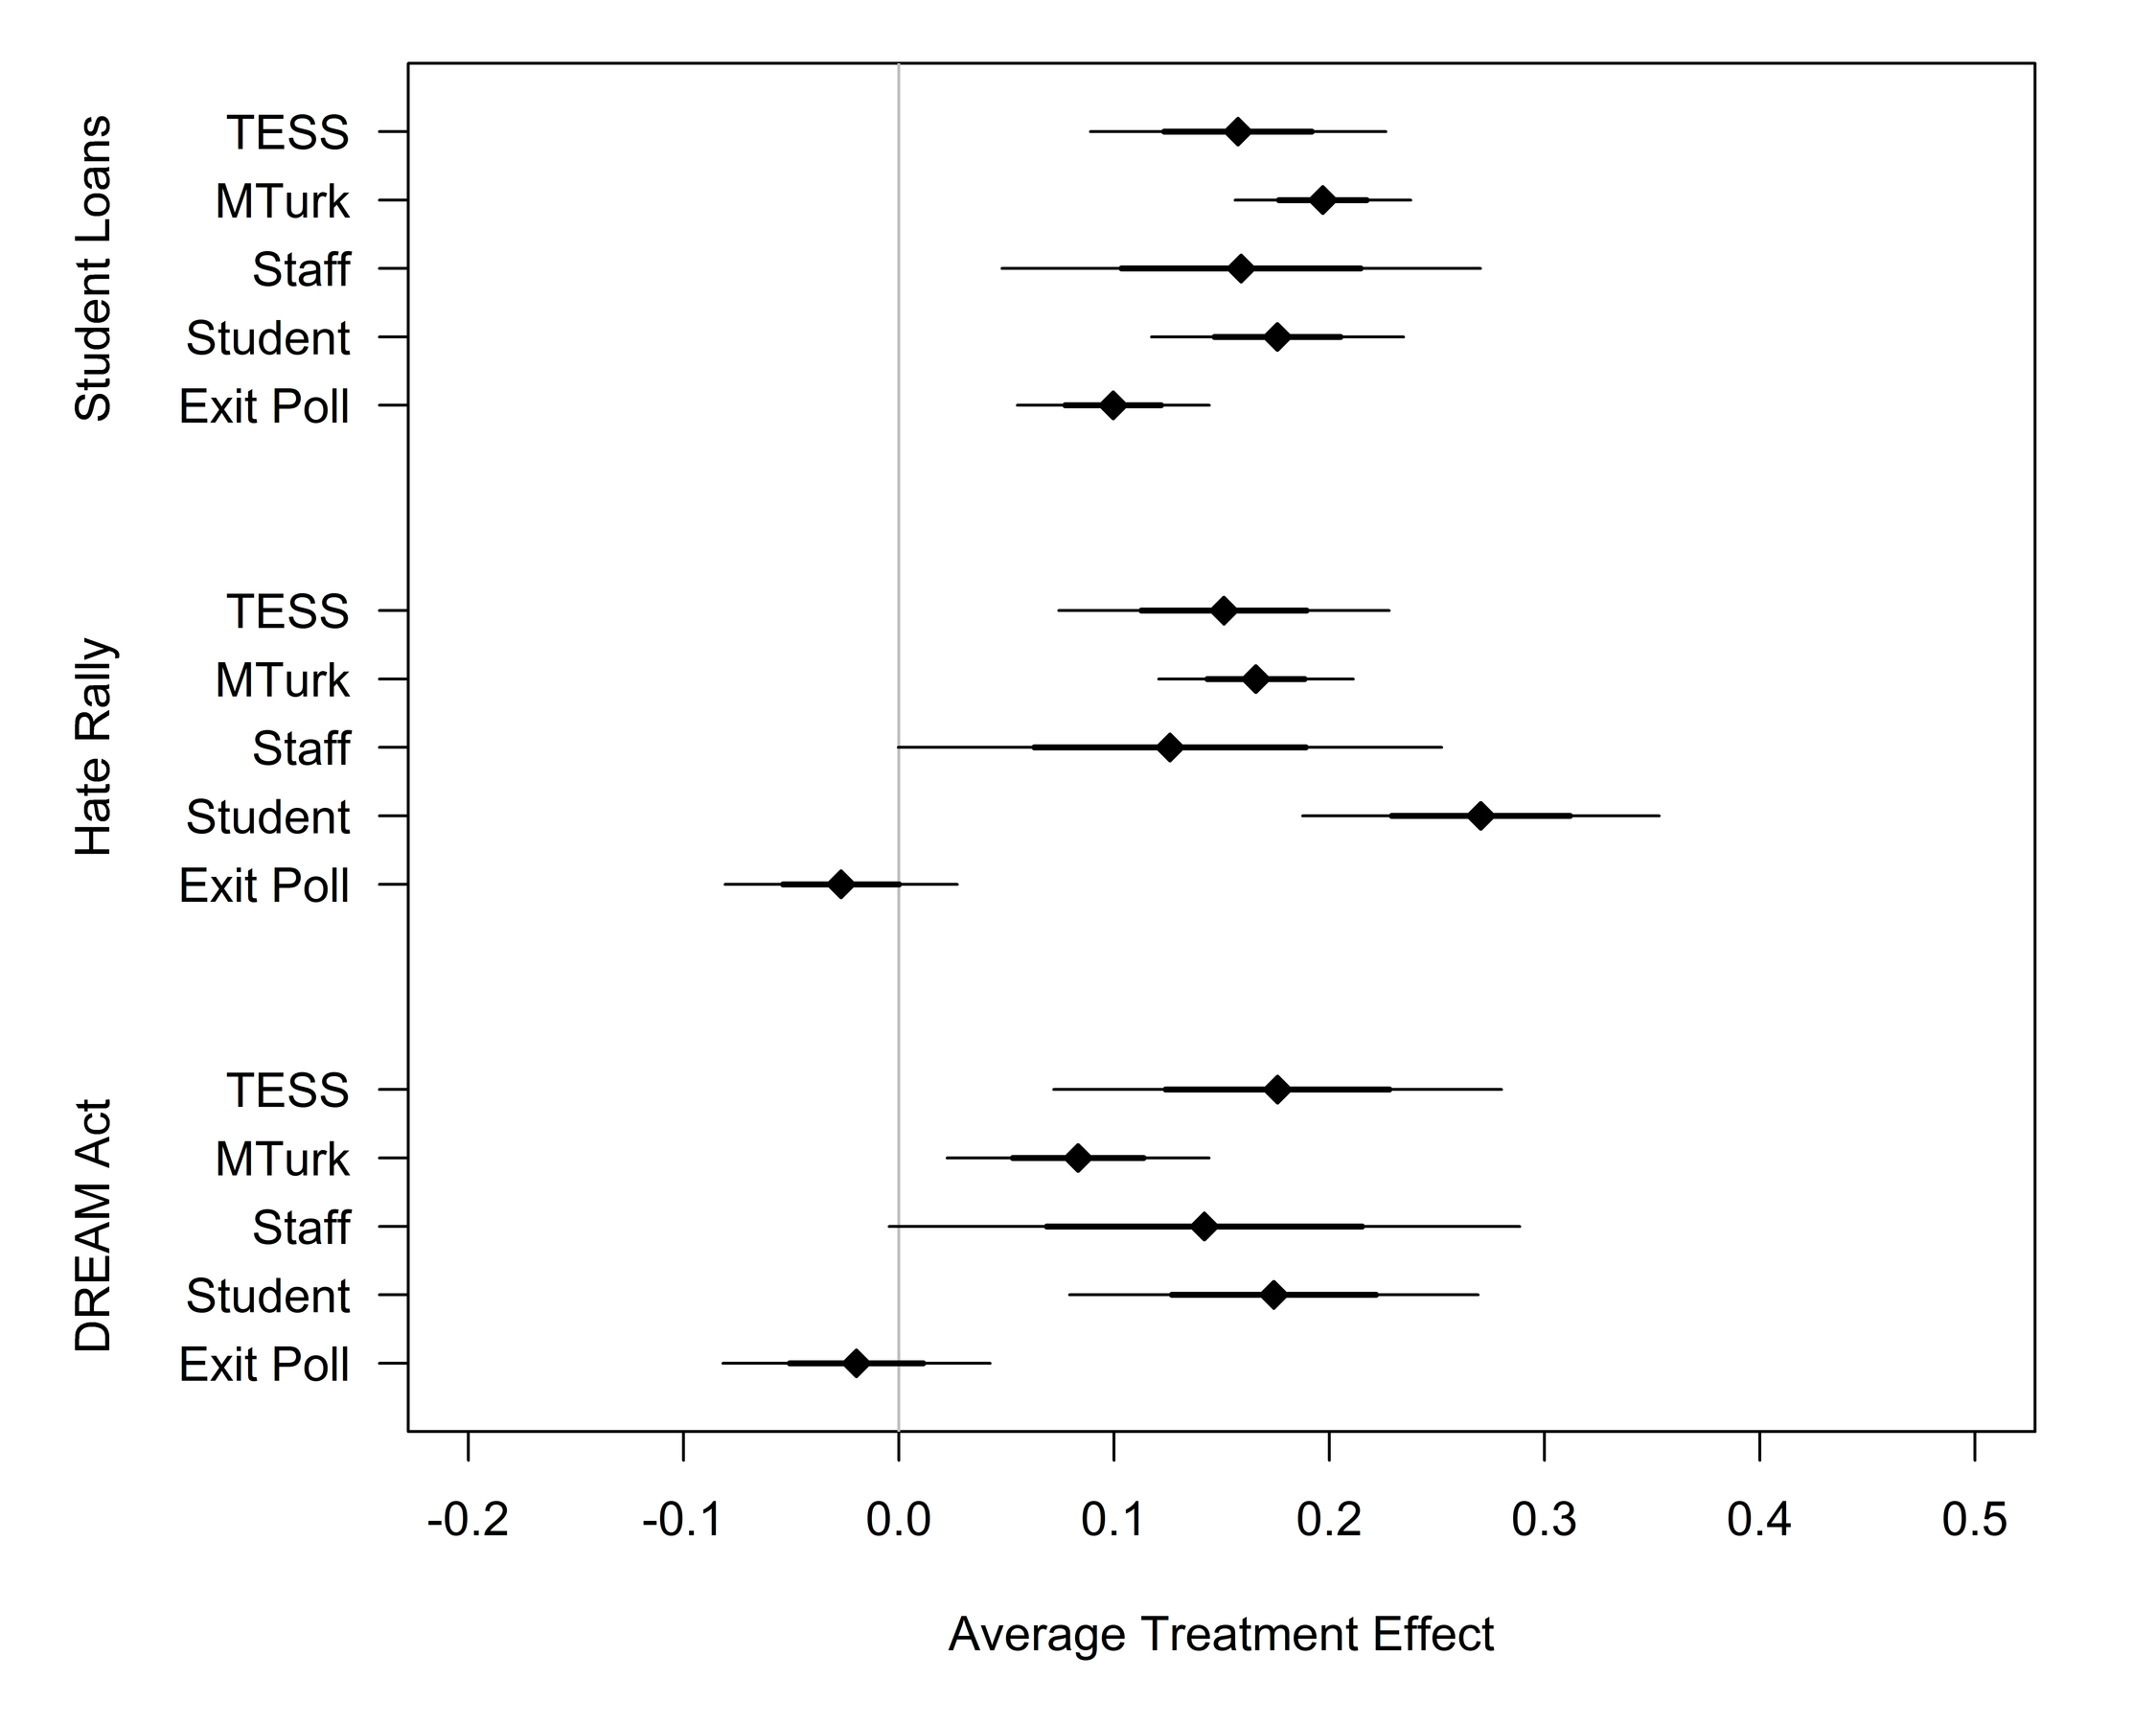
\includegraphics[height=.95\textheight]{images/mullinix3}
\end{center}
}


\frame{
\begin{center}
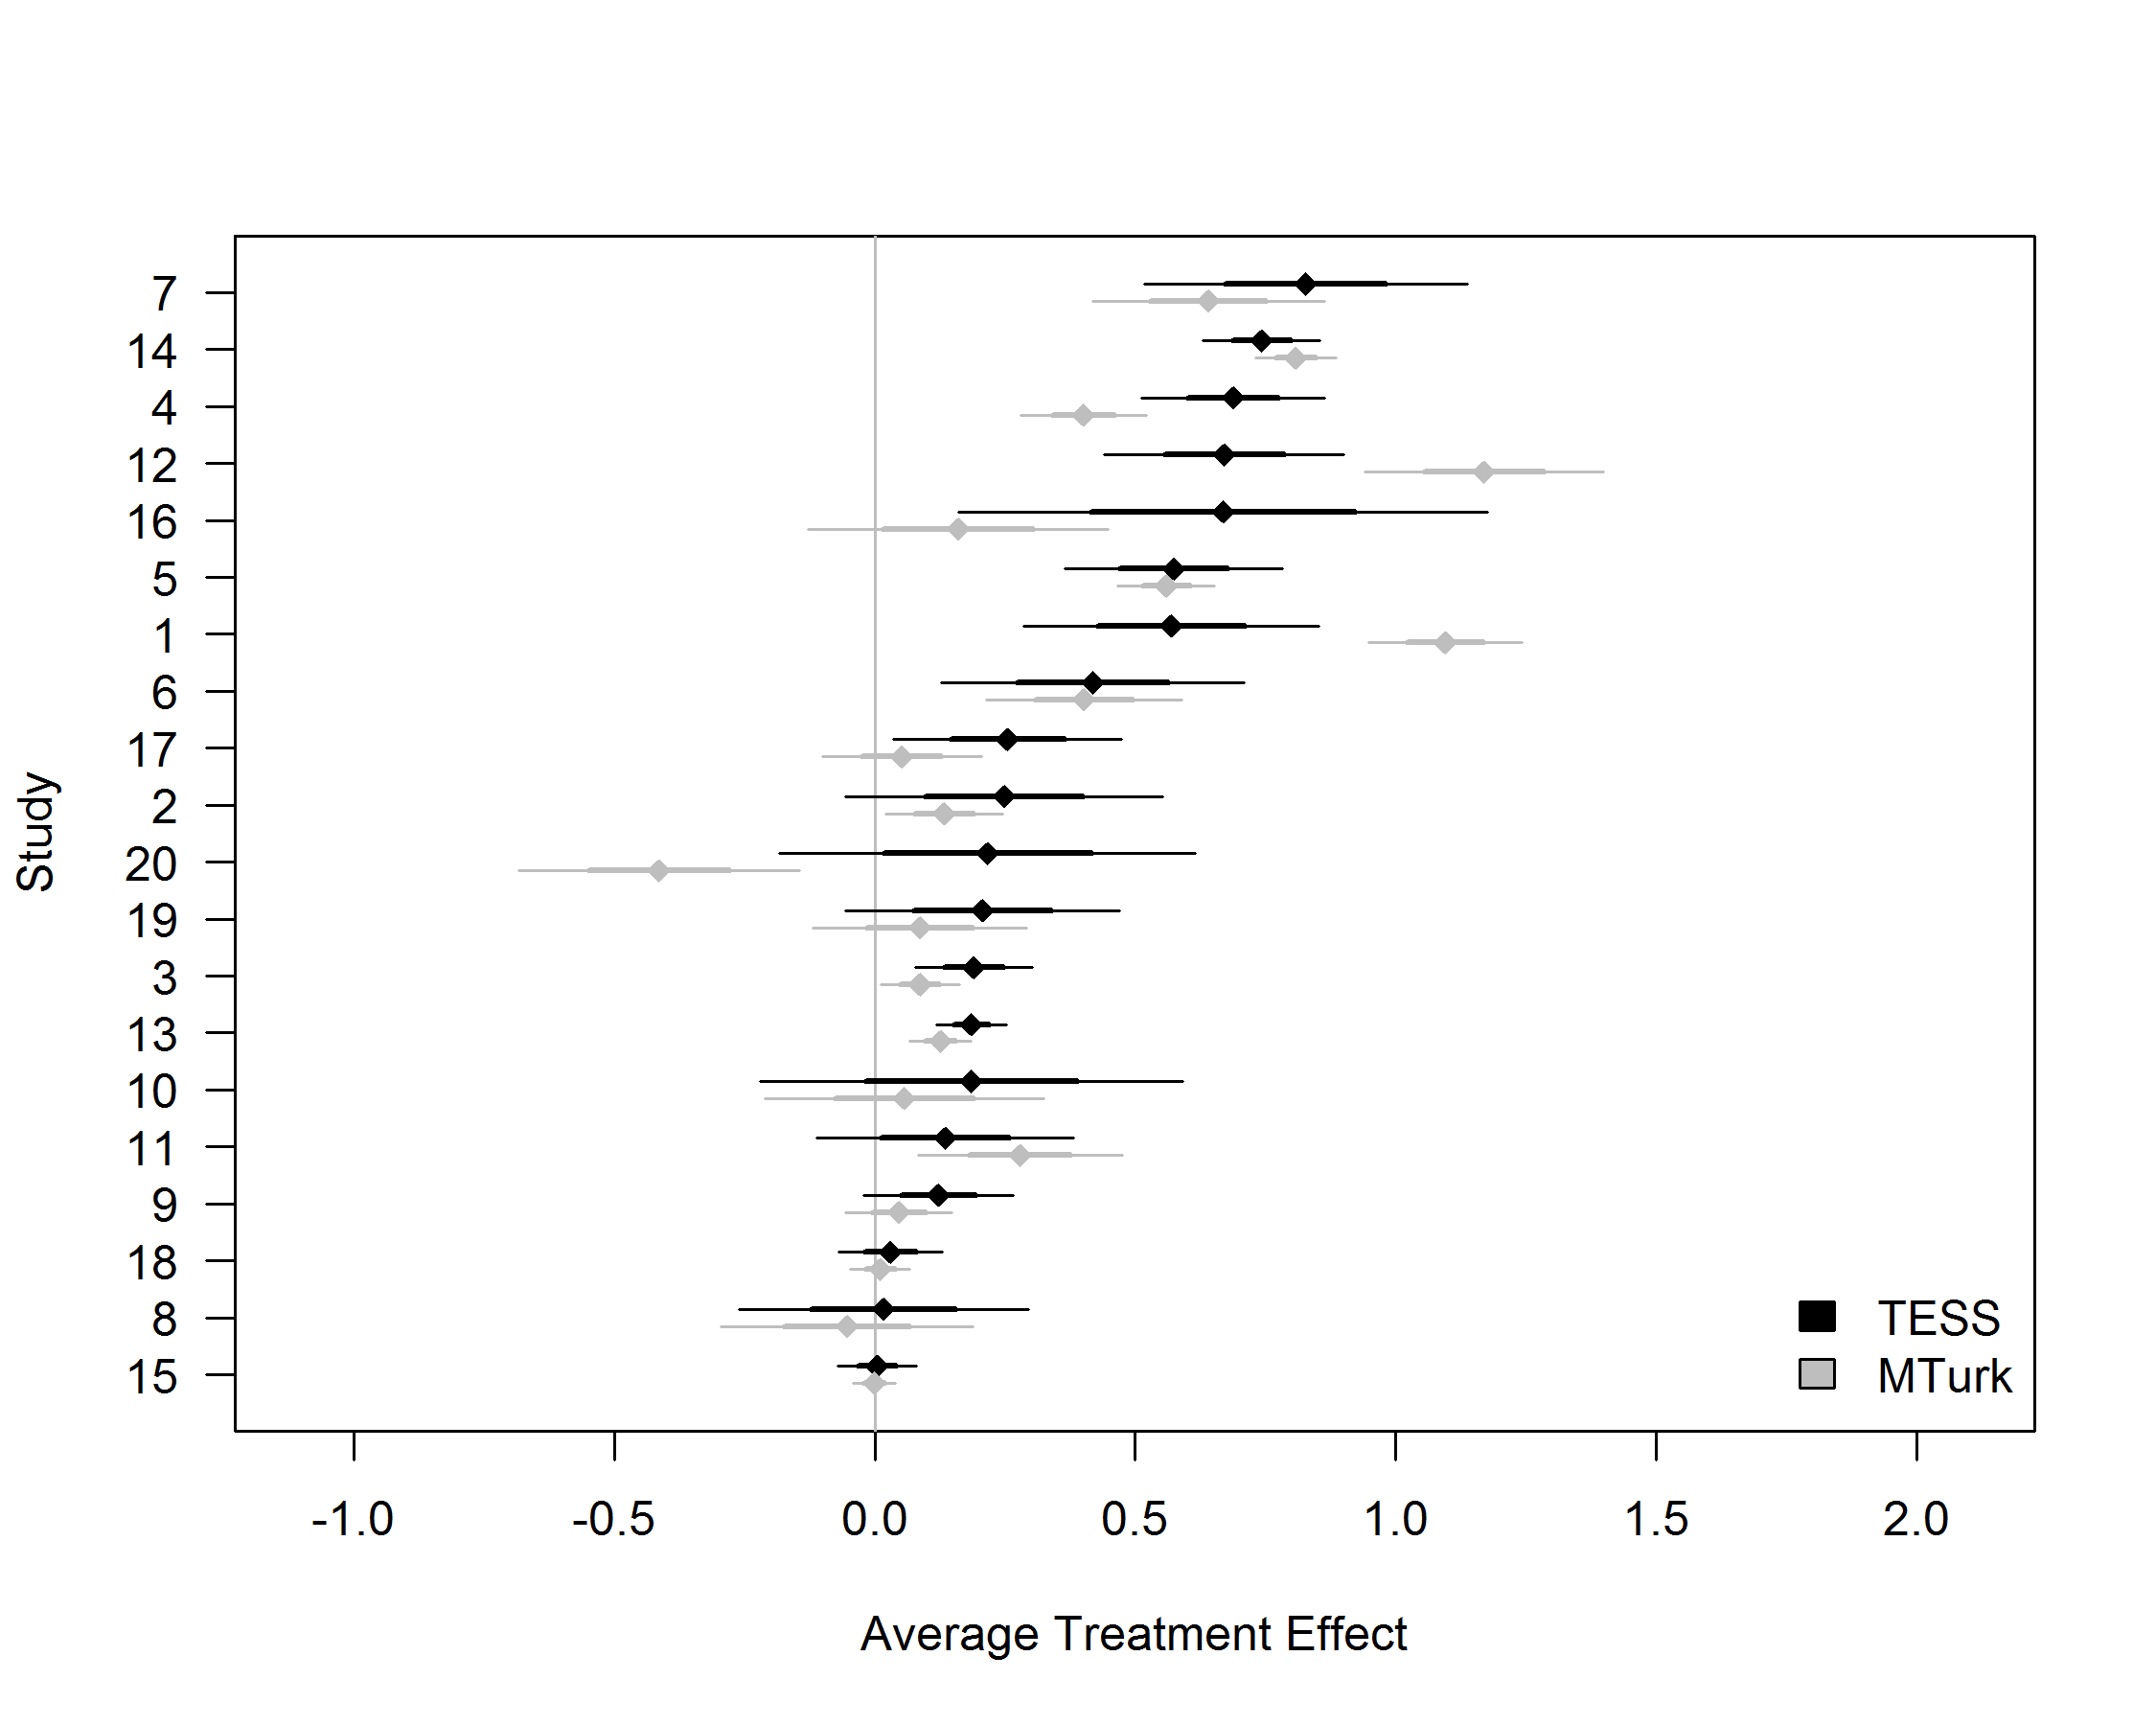
\includegraphics[width=1.1\textheight, trim=0in 0in 0in 0.5in, clip]{images/mullinix1}
\end{center}
}

\againframe<3-4>{myview}

\frame{
\frametitle{SUTO Framework}
\begin{itemize}\itemsep1em
\item Cronbach (1986) talks about generalizability in terms of UTO
\item Shadish, Cook, and Campbell (2001) speak similarly of:
	\begin{itemize}
	\item \textbf{S}ettings
	\item \textbf{U}nits
	\item \textbf{T}reatments
	\item \textbf{O}utcomes
	\end{itemize}
\item External validity depends on all of these things
\end{itemize}
}


\frame{
\begin{columns}[t]
\begin{column}{0.5\textwidth}
	\begin{block}{Population}
		\begin{itemize}
		\item Setting
		\item Units
		\item Treatments
		\item Outcomes
		\end{itemize}
	\end{block}
\end{column}
\begin{column}{0.5\textwidth}
	\begin{block}{Your Study}
		\begin{itemize}
		\item Setting
		\item Units
		\item Treatments
		\item Outcomes
		\end{itemize}
	\end{block}
\end{column}
\end{columns}

\vspace{1em}

\only<2->{In your study, how do these correspond?\\}
\only<3->{\hspace{5.7em} how do these differ?\\}
\only<4->{\hspace{5.7em} do these differences matter?\\}

}


\frame{
\frametitle{Common Differences}
\begin{itemize}\itemsep1em
\item Most common thing to focus on is demographic representativeness
	\begin{itemize}
	\item Sears (1986): ``students aren't real people''
	\item \href{http://www.slate.com/articles/health_and_science/science/2013/05/weird_psychology_social_science_researchers_rely_too_much_on_western_college.html}{Western, educated, industrialized, rich, democratic (WEIRD) psychology participants}
	\end{itemize}
\item<2-> But do those characteristics actually matter?
\item<3-> Shadish, Cook, and Campbell tell us to think about:
	\begin{itemize}
	\item Surface similarities
	\item Ruling out irrelevancies
	\item Making discriminations
	\item Interpolation/extrapolation
	\end{itemize}
\end{itemize}
}


\frame{
\frametitle{Focus on effect heterogeneity}
\begin{itemize}\itemsep1em
\item Think about and make an evidence-based argument for why you think there are (or are not) heterogeneous effects
\item<2-> If you think there is heterogeneity, then we probably do not care about the SATE anyway
	\begin{itemize}
	\item Focus on CATE instead
	\item $E[Y_{1i} | X = 1, Z=z] - E[Y_{0i} | X = 0, Z=z]$
	\end{itemize}
\item<3-> Two formal analytic strategies
	\begin{itemize}
	\item Regression with large number of interactions
	\item Bayesian Additive Regression Trees
	\end{itemize}
\item<4-> But remember: you have to convince reviewers!
\end{itemize}
}



\frame{
\frametitle{BART}
\begin{itemize}\itemsep1em
\item Estimate \textit{conditional average treatment effects}
\item BART is essentially an ensemble machine learning method
\item Iteratively split a sample into more and more homogeneous groups until some threshold is reached using binary (cutpoint) decisions
\item Repeat this a bunch of times, aggregating across results
\end{itemize}
}

\frame{
\begin{center}
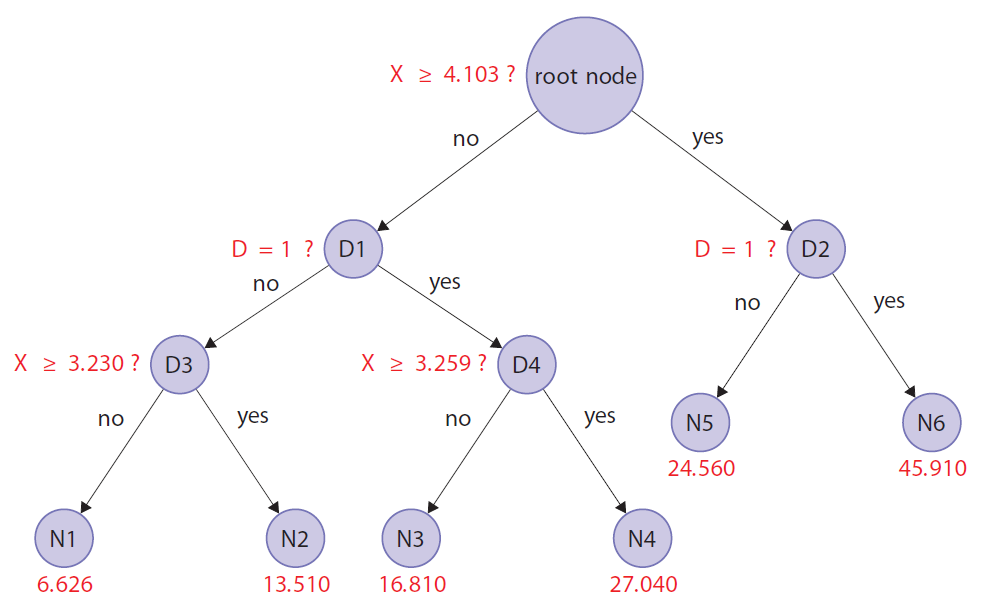
\includegraphics[width=\textwidth]{images/greenkern1}
\end{center}
{\footnotesize Green and Kern. 2012. ``Modeling Heterogeneous Treatment Effects in Survey Experiments with Bayesian Additive Regression Trees.'' \textit{Public Opinion Quarterly}.\par}
}

\frame{
\begin{center}
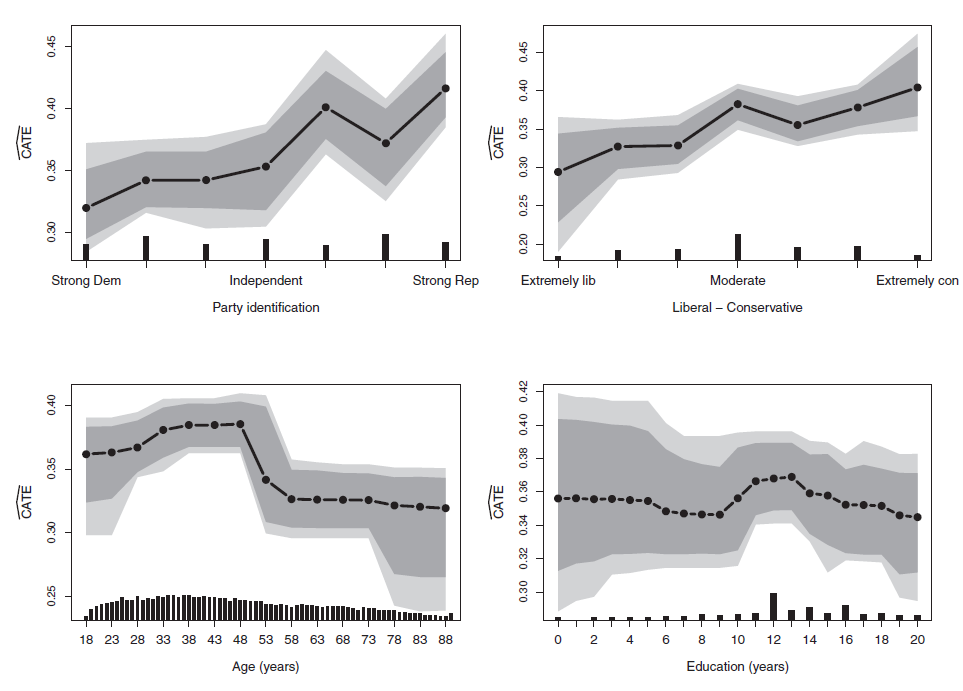
\includegraphics[height=.8\textheight]{images/greenkern2}
\end{center}
{\footnotesize Green and Kern. 2012. ``Modeling Heterogeneous Treatment Effects in Survey Experiments with Bayesian Additive Regression Trees.'' \textit{Public Opinion Quarterly}.\par}
}


\frame{

\frametitle{Stratification/Blocking}

As soon as we care about heterogeneous effects, it makes sense to stratify and block on factors that might moderate the treatment effect.

\vspace{1em}

\onslide<2->{As soon as we identify all sources of heterogeneity, it doesn't matter what sample we use because effects are \textit{by definition} homogeneous within such strata.}

\vspace{1em}

\onslide<3->{But, we never know when we've reached that point!}

}



% induced value theory (swamping preferences)
\frame{
\frametitle{{\large Aside: Induced Value Theory}}
\begin{itemize}\itemsep1em
\item Incentivized (economic) experiments rely on induced value theory
\item This is a way to reduce heterogeneity
	\begin{itemize}
	\item Incentives reduce variation across individuals
	\item Sample characteristics should matter less (than in other types of research)
	\end{itemize}
\item Actually merits empirical testing, though
\end{itemize}
}


\frame{

If we acknowledge and start thinking about effect heterogeneity, does this mean we can use any convenient group of participants as if they were probability samples?

\vspace{1em}

No. Of course not.
}


% defining your convenience sample
\frame{
	\frametitle{Not All Convenience Samples Are Alike}
	\begin{itemize}\itemsep1em
		\item<1-> Different types:
			\begin{itemize}
				\item<2-> Passive/opt-in/``river sampling''
				\item<3-> Sample of convenience (not a sample per se)
					\begin{itemize}
					\item Email list
					\item Snowball sample
					\item Respondent-driven Sampling
					\item Students
					\item Crowdsourcing
					\end{itemize}
			\end{itemize}
		\item<4-> Differ in numerous ways
			\begin{itemize}
			\item Cost
			\item ``Experience''
			\item Attentiveness
			\item Demographics
			\end{itemize}
	\end{itemize}
}

\frame{
\frametitle{Costs per participant}

From one of my studies:\\

\vspace{1em}

\centering
\begin{tabular}{l r r r}
Sample	& Cost	& n	& Cost/participant\\ \midrule
National	& \$13200	& 593	& \$22.26\\
Exit Poll	& \$3000	& 741	& \$4.05\\
Students	& \$0	& 299	& \$0\\
Staff		& \$1280	& 128	& \$10.00\\
MTurk	& \$550	& 1024	& \$0.54\\
Ads		& \$636	& 80		& \$7.95\\
\bottomrule
\end{tabular}
}

\frame{
\frametitle{Participant Experience}

\begin{itemize}\itemsep1em
\item A lot of growing concern about experience
\item Larger literature on ``panel conditioning''
	\begin{itemize}
	\item Inconclusive evidence
	\end{itemize}
\item<3-> Some numbers:
	\begin{itemize}
	\item<3-> MTurk workers are doing 100+ studies per month
	\item<4-> Numbers are the same for YouGov panelists
	\end{itemize}
\end{itemize}

}



% eligibility; duplication; recontacts
\frame{
\frametitle{My Advice}
\begin{itemize}\itemsep1em
\item Only work with enumerated populations
	\begin{itemize}
	\item Each unit is uniquely identifiable
	\end{itemize}
\item<2-> Without this, you risk many things:
	\begin{itemize}
	\item Ambiguous eligibility
	\item Retakes, treatment crossover
	\item No way to evaluate response rates/bias
	\end{itemize}
\item<3-> Know something about your sample
	\begin{itemize}
	\item How does it differ from your target of inference?
	\item What theories or evidence would suggest those differences should matter?
	\item What can you do to adjust or control for those \textit{consequential} differences?
	\end{itemize}
\end{itemize}
}


\frame{
\frametitle{Measure, Measure, Measure}

\vspace{1em}

The only way to evaluate a sample is to know something about it.

\vspace{1em}

The best way to convince reviewers is to rule out irrelevancies.
}


\frame{
\frametitle{Don't forget statistical power\dots}
\begin{center}
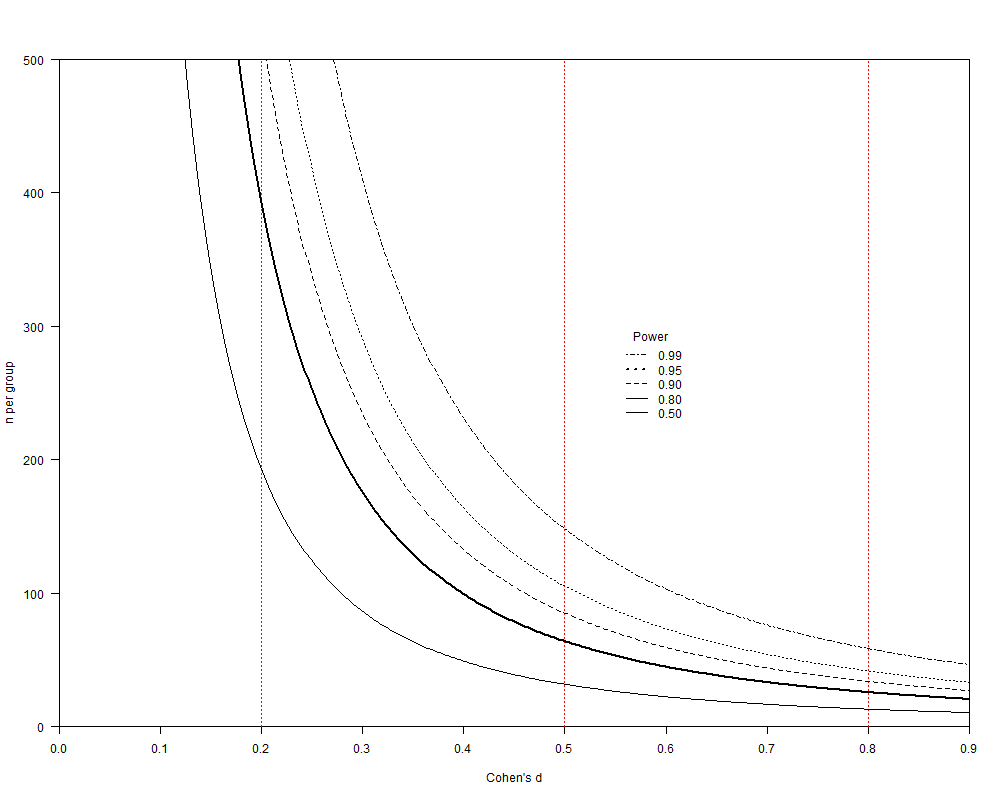
\includegraphics[height=0.85\textheight, trim = 0in 0in 0in 0.5in , clip]{images/power}
\end{center}
}

\frame{}



\section{Web Questionnaires}
\frame{\tableofcontents[currentsection]}

% server-side versus client-side technologies
\frame{

When you navigate to a URL\dots

\begin{center}
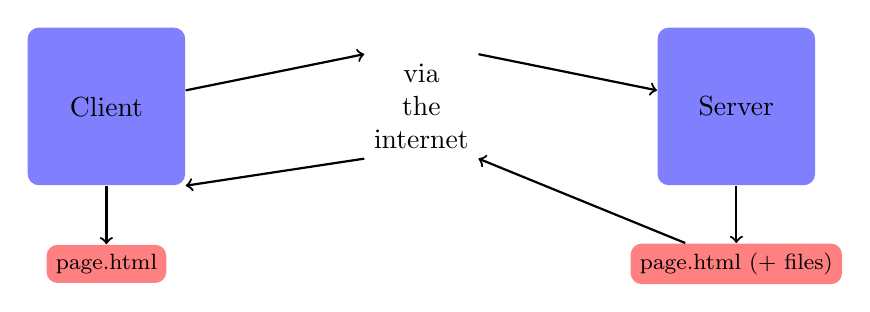
\begin{tikzpicture}
\draw<2-> node[fill=blue!50!white, rounded corners, minimum height=2cm, minimum width=2cm] (client) at (0,0) {Client};
\draw<2-> node[fill=blue!50!white, rounded corners, minimum height=2cm, minimum width=2cm] (server) at (8,0) {Server};
\draw<2-> node[align=center] (internet) at (4,0) {via\\the\\internet};
\draw<2->[thick, ->] (client) -- (internet.north west);
\draw<2->[thick, ->] (internet.north east)-- (server);

\draw<3-> node[fill=red!50!white, rounded corners, align=left] (page) at (8,-2) {{\footnotesize page.html (+ files)}};
\draw<3->[thick, ->] (server) -- (page);

\draw<4->[thick, ->] (page) -- (internet.south east);
\draw<4->[thick, ->] (internet.south west)-- (client.south east);

\draw<5-> node[fill=red!50!white, rounded corners, align=left] (page2) at (0,-2) {{\footnotesize page.html}};
\draw<5->[thick, ->] (client) -- (page2);

\end{tikzpicture}
\end{center}

\small

\begin{enumerate}
\item<2-> your browser sends an HTTP request to a server
\item<3-> the server processes the request and executes server-side code
\item<4-> the server replies with the contents of the page
\item<5-> your browser executes client-side 
\end{enumerate}
}



% what is a web survey?
\frame{

\frametitle{Questionnaires are client side}

A web page consists of four things:

\begin{itemize}
\item HTML describing content
\item Cascading style sheets (CSS) to style that content
\item Images or other multimedia content
\item Javascript code that makes a page dynamic
\end{itemize}

}



\begin{frame}[fragile]
\small
\begin{verbatim}
<html>
<head>
  <title>Survey</title>
</head>
<body>
  <form action="http://httpbin.org/post" method="POST">
    <p>
      <label for="q1">Name: 
        <input type="text" id="q1" name="q1" />
      </label>
    </p>
    <p><input type="submit"></p>
  </form>
</body>
</html>
\end{verbatim}
\end{frame}


% html
% html forms
%% <input type="radio" name="q2" value="1" />
%% <input type="checkbox" name="q2" value="1" />
%% <textarea name="open" rows="10" cols="30">
%% <select name="cars"><option value="volvo">Volvo</option></select>
%% <input type="hidden" />


\frame{
\frametitle{Getting a grip on HTML}
\begin{itemize}\itemsep1em
\item Every element should have an opening \texttt{<tag>} and closing \texttt{</tag>}
\item Necessary tags:
	\begin{itemize}
	\item \texttt{<html></html>}
	\item \texttt{<head></head>}
	\item \texttt{<body></body>}
	\end{itemize}
\item<2-> Use an intelligent text editor (\textit{not Notepad})
\item<3-> Use a validator: \url{https://validator.w3.org/nu/}
\item<4-> Remember that browsers differ
\end{itemize}
}


\bgroup
\setbeamercolor{background canvas}{bg=blue!20!white}
\setbeamertemplate{navigation symbols}{}
\begin{frame}[plain]{}
\begin{center}
\textbf{{\Large Test Yourself!}}

\vspace{2em}

Make a simple complete HTML document that passes displays a paragraph of text and passes the validator

\vspace{2em}

\url{https://validator.w3.org/nu/}
\end{center}
\end{frame}
\egroup





\frame{
\frametitle{Getting a grip on HTML}
\begin{itemize}\itemsep1em
\item Common elements
	\begin{itemize}
	\item \texttt{<div></div>}
	\item \texttt{<span></span>}
	\item \texttt{<p></p>}
	\item \texttt{<h1>}, \texttt{<h2>}, \dots
	\item \texttt{<br />}
	\end{itemize}
\item Tag attributes describe each element:
	\begin{itemize}
	\item \texttt{id}: unique identifier for each element
	\item \texttt{class}: grouping identifier for elements (useful for CSS)
	\item \texttt{style}: in-line CSS styling
	\end{itemize}
\end{itemize}
}





\frame{
\frametitle{Getting a grip on HTML}
\begin{itemize}\itemsep1em
\item Common form elements
	\begin{itemize}
	\item \texttt{<form></form>}
	\item \texttt{<input />}
	\item \texttt{<label></label>}
	\item \texttt{<button />}
	\end{itemize}
\item<2-> Attributes specific to form elements
	\begin{itemize}
	\item \texttt{type}: the kind of input
		\begin{itemize}
		\item ``radio''
		\item ``checkbox''
		\item ``text''
		\end{itemize}
	\item \texttt{name}: the ``variable'' being recorded
	\item \texttt{value}: the default variable value
	\end{itemize}
\end{itemize}
}



\bgroup
\setbeamercolor{background canvas}{bg=blue!20!white}
\setbeamertemplate{navigation symbols}{}
\begin{frame}[plain]{}
\begin{center}
\textbf{{\Large Test Yourself!}}

\vspace{2em}

Make a simple HTML form that displays a question and a free response answer and passes the validator

\vspace{2em}

\url{https://validator.w3.org/nu/}
\end{center}
\end{frame}
\egroup



\bgroup
\setbeamercolor{background canvas}{bg=blue!20!white}
\setbeamertemplate{navigation symbols}{}
\begin{frame}[plain]{}
\begin{center}
\textbf{{\Large Test Yourself!}}

\vspace{2em}

Make a simple HTML form that displays a question and a multiple choice answer and passes the validator

\vspace{2em}

\url{https://validator.w3.org/nu/}
\end{center}
\end{frame}
\egroup



\frame{

Some other elements:

\begin{itemize}
\item Bullet list: \texttt{<ul></ul>}
\item Enumerated list: \texttt{<ol></ol>}
	\begin{itemize}
	\item List element: \texttt{<li></li>}
	\end{itemize}
\item Tables:
	\begin{itemize}
	\item Table: \texttt{<table></table>}
	\item Header: \texttt{<th></th>}
	\item Row: \texttt{<tr></tr>}
	\item Cell: \texttt{<td></td>}
	\end{itemize}
\end{itemize}

}




% css
\frame{
\frametitle{Getting a grip on HTML}

HTML files can also contain other content

\begin{itemize}\itemsep1em 
\item Style sheets (CSS) in \texttt{<style></style>} elements in head
\item Javascript in \texttt{<script></script>} elements in head and/or body
\item Images (\texttt{<img src="url" />})
\item HTML5 features (e.g., \texttt{<canvas>}, \texttt{<svg>})
\end{itemize}
}


\frame<1>[label=css]{
\frametitle{CSS is Elegant}

\begin{itemize}\itemsep1em
\item HTML originally (until 1996) had to be styled manually
\item<2-> CSS allows you to style a document separately from its content
	\begin{itemize}
	\item Class- and element-specific styling
	\item Change styling without changing the HTML
	\end{itemize}
\item<3-> Can be included inline, in \texttt{<head>}, or in separate document
\end{itemize}

}


\frame{
\begin{columns}
\column{\dimexpr\paperwidth-15pt}
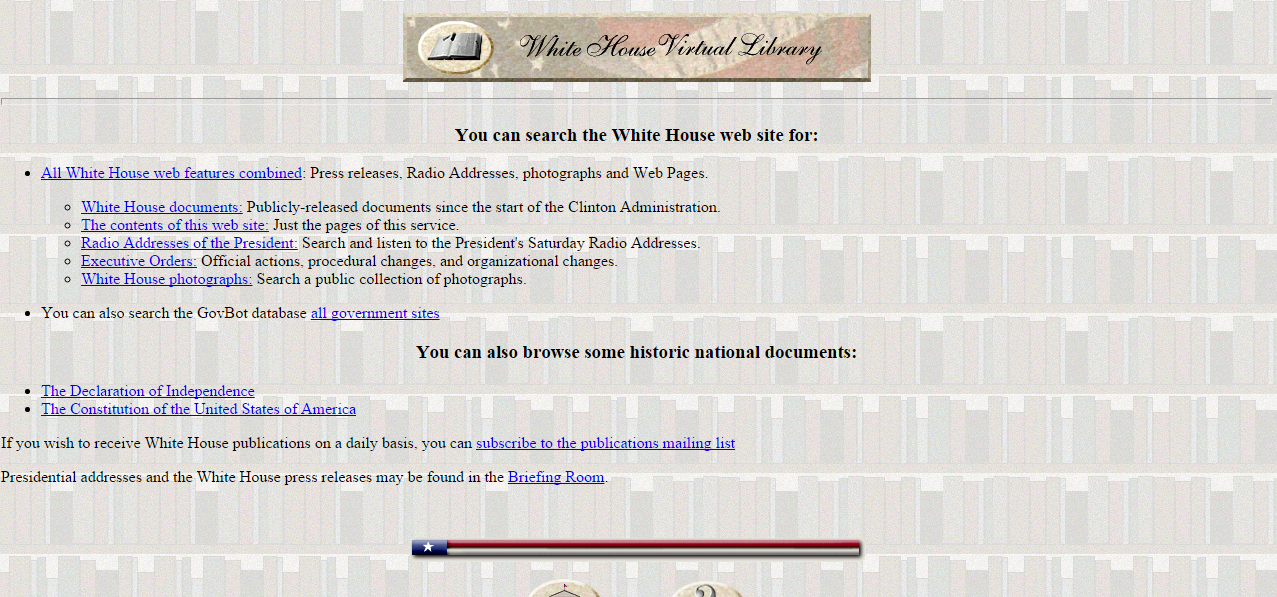
\includegraphics[width=1.2\textwidth]{images/whitehouse}
\end{columns}
}

\againframe{css}



\bgroup
\setbeamercolor{background canvas}{bg=blue!20!white}
\setbeamertemplate{navigation symbols}{}
\begin{frame}[plain]{}
\begin{center}
\textbf{{\Large Test Yourself!}}

\vspace{2em}

Make a simple HTML form uses CSS to style the answer options to your past survey and passes the validator

\vspace{2em}

\url{https://validator.w3.org/nu/}
\end{center}
\end{frame}
\egroup



% javascript for randomized redirect
\begin{frame}[fragile]
\small
\begin{verbatim}
<html>
<head>
  <title>Redirect</title>
</head>
<body>
  <script>
  var u = new Array ();
  u[0] = "http://www.google.com";
  u[1] = "http://www.bing.com";
  u[2] = "http://www.yahoo.com";
  var i = Math.floor(u.length*Math.random());
  document.write("Redirecting to " + u[i]);
  window.location.replace(u[i]);
  </script>
</body>
</html>
\end{verbatim}
\end{frame}



% javascript for randomized display of a link
\begin{frame}[fragile]
\small
\begin{verbatim}
<html>
<head>
  <title>Redirect</title>
</head>
<body>
  <p>Please read the following:</p>
  <script>
  var u = new Array ();
  u[0] = "Treatment 1";
  u[1] = "Treatment 2";
  u[2] = "Treatment 3";
  var i = Math.floor(u.length*Math.random());
  document.write("<p><b>" + u[i] + "</b></p>");
  </script>
</body>
</html>
\end{verbatim}
\end{frame}



\bgroup
\setbeamercolor{background canvas}{bg=blue!20!white}
\setbeamertemplate{navigation symbols}{}
\begin{frame}[plain]{}
\begin{center}
\textbf{{\Large Test Yourself!}}

\vspace{2em}

Make a simple HTML form that displays a randomly selected piece of text and passes the validator

\vspace{2em}

\url{https://validator.w3.org/nu/}
\end{center}
\end{frame}
\egroup



% javascript for youtube video presentation
\begin{frame}[fragile]
\tiny
\begin{verbatim}
<html>
<head>
  <title>Survey</title>
</head>
<body>
  <div id="player"></div>
  <script>
  var tag = document.createElement('script'); 
  tag.src = "https://www.youtube.com/iframe_api";
  var firstScriptTag = document.getElementsByTagName('script')[0];
  firstScriptTag.parentNode.insertBefore(tag, firstScriptTag);
  
  var player;
  function onYouTubeIframeAPIReady() {
    player = new YT.Player('player', {
      height: '390',
      width: '640',
      videoId: '0Bmhjf0rKe8',
      playerVars: {
        'controls': '0',
        'showinfo': '0',
        'rel': '0'
      },
      events: {
        'onReady': onPlayerReady
      }
    });
  }
  
  function onPlayerReady(event) {
    event.target.playVideo();
  }
  </script>
  
</body>
</html>
\end{verbatim}
\end{frame}





\frame{

\Large

If client-side is so cool\dots\\

\vspace{1em}

\dots why do we care about server-side technology?

}

\frame{
\begin{columns}[t]
\begin{column}{0.5\textwidth}
	\begin{block}{Client-Side}
		\begin{itemize}
		\item<2-> HTML (markup)
		\item<2-> CSS (styling)
		\item<2-> Javascript (scripting)
		\end{itemize}
	\end{block}
\end{column}
\begin{column}{0.5\textwidth}
	\begin{block}{Server-Side}
		\begin{itemize}
		\item<3-> Python, PHP, \dots
		\item<3-> Cookies
		\item<3-> Databases
		\end{itemize}
	\end{block}
\end{column}
\end{columns}

\vspace{1em}

\only<4->{We need a server to record a participant's behavior}

}


% 

\bgroup
\setbeamercolor{background canvas}{bg=blue!20!white}
\setbeamertemplate{navigation symbols}{}
\begin{frame}[plain]{}
\frametitle{Web Questionnaires}
\begin{itemize}\itemsep1em
\item Google Spreadsheet Forms:\\
	\url{https://www.google.co.uk/forms/about/}
\item Survey Monkey:\\ 
	\url{https://www.surveymonkey.com/home/}
\item Qualtrics:\\
	\url{https://www.qualtrics.com/login/}
\end{itemize}
\end{frame}
\egroup



% Google Spreadsheet forms

\frame{
\frametitle{Web Questionnaires}
\begin{itemize}\itemsep1em
\item Google Spreadsheet Forms:\\
\url{https://www.google.co.uk/forms/about/}
\item Features
	\begin{itemize}
	\item Free!
	\item Somewhat complex branching
	\item No randomization
	\end{itemize}
\end{itemize}
}


\frame{
\frametitle{Google Consumer Surveys}
\begin{itemize}\itemsep1em
\item \url{http://www.google.com/insights/consumersurveys/home}
\item Features
	\begin{itemize}
	\item Cheap and fast
	\item Very limited functionality
	\item One-off questionnaires
	\item Great for pilot testing
	\end{itemize}
\end{itemize}
}


\frame{
\frametitle{Survey Monkey}
\begin{itemize}\itemsep1em
\item \url{https://www.surveymonkey.com/home/}
\item Features
	\begin{itemize}
	\item Free account
	\item Limited surveys and respondents
	\item No randomization in free account
	\item Nice respondent management tools (``collectors'')
	\end{itemize}
\end{itemize}
}


\bgroup
\setbeamercolor{background canvas}{bg=blue!20!white}
\setbeamertemplate{navigation symbols}{}
\begin{frame}[plain]{}
\begin{center}
\textbf{{\Large Test Yourself!}}

\vspace{2em}

Create a simple survey and create a panel including yourself and maybe me (\href{mailto:thosjleeper@gmail.com}{thosjleeper@gmail.com}) as recipients. Try sending the survey.

\end{center}
\end{frame}
\egroup



\frame{
\frametitle{Qualtrics}
\begin{itemize}\itemsep1em
\item \url{https://www.qualtrics.com/login/}
\item Features
	\begin{itemize}
	\item Free account w/ limited surveys and respondents
	\item Much more expensive than SurveyMonkey
	\item Powerful randomization functionality
	\item Useful ``embedded data'' controls
	\item Optimized for mobile
	\end{itemize}
\end{itemize}
}

\bgroup
\setbeamercolor{background canvas}{bg=blue!20!white}
\setbeamertemplate{navigation symbols}{}
\begin{frame}[plain]{}
\begin{center}
\textbf{{\Large Test Yourself!}}
\end{center}

\vspace{2em}

Create two kinds of randomization: 

\begin{enumerate}
\item Using a random embedded data field
\item Using block randomization
\end{enumerate}

Preview the survey to make sure it works.

\end{frame}
\egroup




% show off how to link MTurk
\begin{frame}[fragile]
\frametitle{Connecting Surveys to MTurk}

\tiny
\begin{verbatim}
<html>
<head></head>
<body>
  <script>
  function turkGetParam( name ) { 
    var regexS = "[\?&]"+name+"=([^&#]*)"; 
    var regex = new RegExp( regexS ); 
    var tmpURL = window.location; 
    var results = regex.exec( tmpURL ); 
    if( results == null ) { 
      return ""; 
    } else { 
      return results[1];    
    } 
  }
  var assign = turkGetParam('assignmentId');
  var worker = turkGetParam('workerId');
  var surveylink = new String("http://httpbin.org/get?"+"assignmentId="+assign+"&workerId="+worker);
  if(assign=="ASSIGNMENT_ID_NOT_AVAILABLE") {
      /* DO NOTHING */
  }
  else {
      document.write("<p>Visit <a href='" + surveylink + "' target='_blank'>this link</a></p>");
  }
  </script>
  <form action="http://httpbin.org/post">
    <p><label for="code">Code: <input type="text" id="code" name="code" /></label></p>
    <p><input type="submit"></p>
  </form>
</body>
</html>
\end{verbatim}
\end{frame}



\bgroup
\setbeamercolor{background canvas}{bg=blue!20!white}
\setbeamertemplate{navigation symbols}{}
\begin{frame}[plain]{}
\begin{center}
\textbf{{\Large Test Yourself!}}

\vspace{2em}

Setup an embedded data field in Qualtrics and then use a webform or simple hyperlink to redirect someone to your survey using that embedded data field.

\vspace{1em}

Try out the form (or link) and see how it is registered in your Qualtrics data.

\end{center}
\end{frame}
\egroup



% design considerations
% loss of control (mobile platforms; text size; images; videos; different browsers)
% know your sample

\frame<1>[label=design]{
\frametitle{Design Considerations}
\begin{itemize}\itemsep1em
\item Qualtrics highlights challenge of modern devices
\item<2-> But it's not just device size
	\begin{itemize}
	\item Different browsers
	\item Readability
	\item Images/video
	\end{itemize}
\item<3-> Web represents a general loss of control
\item<4-> So, key is know your sample before you use it
\end{itemize}
}


\frame{
\begin{center}
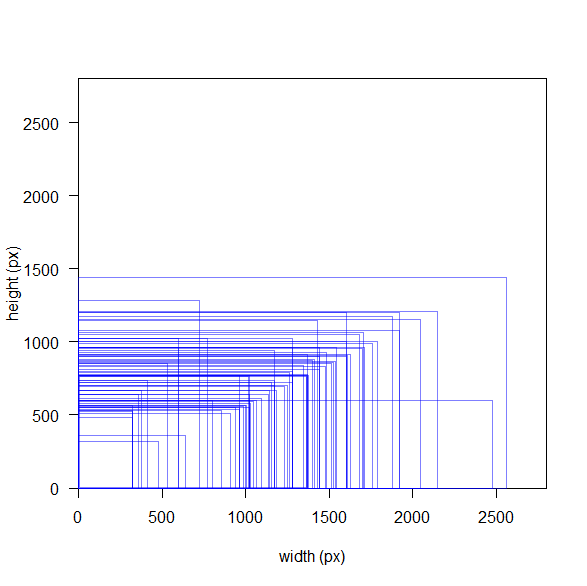
\includegraphics[height=.9\textheight]{images/devicesizes}
\end{center}
}

\againframe{design}

% pretesting everything
\frame{
\frametitle{Two flavors of pretesting}
\begin{enumerate}\itemsep2em
\item Technical pretesting
	\begin{itemize}
	\item Make sure your instrument works
	\item Across browsers/platforms/devices
	\end{itemize}
\item Substantive pretesting
	\begin{itemize}
	\item Does your instrument make sense
	\item Does it make sense for your participants
	\end{itemize}
\end{enumerate}
}







% custom/bespoke solutions
% heroku/otree









\section[Recruitment]{Recruitment in Practice}
\frame{\tableofcontents[currentsection]}


\frame{
\frametitle{{\large For Multi-Person Games}}
\begin{itemize}\itemsep1em
\item Simultaneous participation can be challenging
\item Best workflow is lab-like:
	\begin{enumerate}
	\item Recruit participants
	\item Schedule them for time slots
	\item Monitor to ensure participants show up
	\item Pay a show-up fee
	\end{enumerate}
\item So, think of the following as relevant to the first two steps in that process
%\item We'll talk more about running multi-person sessions later
\end{itemize}
}


\frame{}


\frame{
\frametitle{Professional Panels}
\begin{itemize}\itemsep1em
\item Big players: SSI, YouGov, GfK, TNS/Gallup
\item Online panels of respondents
\item Respondents participate for incentives
\item Study costs are negotiated
	\begin{itemize}
	\item Sample size
	\item Study length (number of survey items)
	\item Targetting
	\item Timing
	\end{itemize}
\end{itemize}
}

\frame{
\frametitle{Considerations}
\begin{itemize}\itemsep0.75em
\item Recruitment
	\begin{itemize}
	\item Sampling
	\item Opt-in
	\item A mix of each
	\end{itemize}
\item Incentives
\item Frequency of participation
\item ``Profile'' variables
\item Quotas, post-stratification, weighting
\item Respondent ``quality''
\end{itemize}
}


% YouGov sample matching method
\frame{
\frametitle{{\large KnowledgeNetworks versus YouGov}}
\begin{itemize}\itemsep1em
\item Big debate in early 2000s about online panels
	\begin{itemize}
	\item KN used ABS to build a representative panel
	\item YouGov created an opt-in panel; used ``sample matching''
	\end{itemize}
\item<2-> YouGov's process:
	\begin{itemize}
	\item Randomly sample from a list
	\item Match each sampled individual to someone in their opt-in panel
	\item Survey the matched individuals
	\end{itemize}
\item<3-> Evidence inconclusive but many think KN approach is better
\end{itemize}
}


\frame{
\frametitle{Opt-in Crowdsourcing Sites}
\begin{itemize}\itemsep1em
\item Not exactly a panel (fully opt-in)
\item Incentivized participation
\item<2-> Prominent examples
	\begin{itemize}
	\item MTurk
	\item Crowdflower
	\item Microworkers
	\item Prolific Academic
	\end{itemize}
\end{itemize}
}


% Mturk
% Crowdflower
% Microworkers
% Prolific Academic
% Others
%% Click worker
%%


\frame{}


\bgroup
\setbeamercolor{background canvas}{bg=blue!20!white}
\setbeamertemplate{navigation symbols}{}
\begin{frame}[plain]{}
\begin{center}
\textbf{{\Large Test Yourself!}}

\vspace{2em}

Use one of the sites we discussed to setup a basic study invitation.

\vspace{1em}

Probably best to try Crowdflower or Prolific Academic.

\end{center}
\end{frame}
\egroup



\frame{
\frametitle{Other Recruitment Methods}
\begin{itemize}\itemsep1em
\item Online advertising
\item Webforums
\item Email lists (students, staff, etc.)
\end{itemize}
}

% randomizing an email list

\frame{
\frametitle{Randomization}
\begin{itemize}\itemsep1em
\item Two flavors of randomness
\item Pseudo-random
	\begin{itemize}
	\item Not actually random
	\item Reproducible
	\item Implemented everywhere
	\item Excel: \texttt{=RANDBETWEEN(1,3)}
	\item R: \texttt{sample(1:3, 100, TRUE)}
	\end{itemize}
\item Truly random
	\begin{itemize}
	\item Not reproducible
	\item \url{http://www.random.org/}
	\end{itemize}
\end{itemize}
}



\frame{}

% Transparency/Reproducibility

\frame{
\frametitle{Open Science Considerations}
\begin{itemize}\itemsep1em
\item Regardless of how you run studies, try to make them \textit{reproducible}
\item What does this mean?
\item Why do we care?
\end{itemize}
}

\frame{
\frametitle{Reproducibility}
\begin{itemize}\itemsep1em
\item<2-> Everything you do for your study should be publicly shared after publication
	\begin{itemize}
	\item \href{http://www.dataverse.org}{Dataverse}
	\item \href{http://osf.io}{Open Science Framework}
	\item \href{http://figshare.com}{figshare}
	\end{itemize}
\item<3-> This helps others build on your work
\item<4-> Makes it easier for you to build on your work
\item<5-> Makes you a more careful researcher
\end{itemize}
}

\frame{
\frametitle{Some Examples}

\begin{itemize}\itemsep1em
\item Leeper, Thomas J. 2014. ``The Informational Basis for Mass Polarization.'' \textit{Public Opinion Quarterly} 78(1): 27--46.
	\begin{itemize}
	\item On Dataverse: \url{http://hdl.handle.net/1902.1/21964}
	\end{itemize}
\item Mullinix, Kevin J., Leeper, Thomas J., Druckman, James N., and Freese, Jeremy. 2015. ``The Generalizability of Survey Experiments.'' \textit{Journal of Experimental Political Science}: In press.
	\begin{itemize}
	\item On Dataverse: \url{http://dx.doi.org/10.7910/DVN/MUJHGR}
	\end{itemize}
\end{itemize}
}


\frame{
\frametitle{What should be shared?}
\begin{itemize}
\item Recruitment protocol and materials
\item Complete questionnaire (plain text)
\item Web forms/markup
\item Data (raw, but anonymized)
\item Codebook
\item Data Preparation Code
\item Analysis Code
\item Manuscript pre-print
\item Preanalysis plan (if applicable)
\item README
\end{itemize}
}


\frame{
\frametitle{Some Reproducibility Tips}
\begin{enumerate}\itemsep1em
\item<2-> Be selfish\onslide<3->{: Be reproducible for yourself first; benefits for science are a positive externality}
\item<4-> Start early\onslide<5->{: Develop a reproducible workflow from day 1}
\item<6-> Save everything\onslide<7->{: Archive frequently so you never lose your work}
\end{enumerate}
}


\frame{}




% apps
\frame{
\frametitle{Developing Custom Apps}
\begin{itemize}\itemsep1em
\item<1-> Apps provide much more data than HTML forms
	\begin{itemize}
	\item Geolocation
	\item Accelerometer (and other sensors)
	\item User account data (with permissions)
	\end{itemize}
\item<2-> MIT AppInventor: \url{http://appinventor.mit.edu/}
\item<2-> Trinity edX course (\href{https://courses.edx.org/courses/course-v1\%3ATrinityX\%2BT002x\%2B3T2015/}{link})
\end{itemize}

}


\frame{}


\section{Challenges and Opportunities}
\frame{\tableofcontents[currentsection]}

\frame{}


% reweighting; pscore methods
\frame{
\frametitle{Reweighting}
\begin{itemize}\itemsep1em
\item It may be possible to \textit{reweight} convenience sample data to match a population
\item Any method for this is ``model-based'' (rather than ``design-based'')
\item Not widely used or evaluated (yet)
\item All techniques build on the idea of stratification
\end{itemize}
}


\frame{
	\frametitle{Overview of Stratification}
	\begin{enumerate}\itemsep0.5em
		\item Define population
		\item Construct a sampling frame
		\item Identify variables we already know about units in the sampling frame
		\item Stratify sampling frame based on these characteristics
		\item Collect an SRS (of some size) within each stratum
		\item Aggregate our results
	\end{enumerate}
}

\frame{
	\frametitle{Estimates from a stratified sample}
	\begin{itemize}\itemsep0.5em
		\item Within-strata estimates are calculated just like an SRS
		\item Within-strata variances are calculated just like an SRS
		\vspace{1em}
		\item Sample-level estimates are weighted averages of stratum-specific estimates
		\item Sample-level variances are weighted averages of strataum-specific variances
	\end{itemize}
}


\frame{
	\frametitle{Post-Stratification}
	\begin{itemize}\itemsep1em
		\item Used to correct for nonresponse, coverage errors, and sampling errors
		\item<2-> Reweight sample data to match population distributions
			\begin{itemize}
				\item Divide sample and population into strata
				\item Weight units in each stratum so that the weighted sample stratum contains the same proportion of units as the population stratum does
			\end{itemize}
		\item<3-> There are numerous other related techniques
	\end{itemize}
}

\frame{
	\frametitle{Post-Stratification: Example}
	\begin{itemize}\itemsep1em
		\item Imagine our sample ends up skewed on immigration status and gender relative to the population\\
		\vspace{1em}
		\small
		\begin{tabular}{lrrlr}
			\hline
			Group             & Pop. & Sample & Rep.                &              Weight \\ \hline
			Native-born, Female    &  .45 &     .5 & \onslide<2->{Over}  & \onslide<3->{0.900} \\
			Native-born, Male      &  .45 &     .4 & \onslide<2->{Under} & \onslide<4->{1.125} \\
			Immigrant, Female &  .05 &    .07 & \onslide<2->{Over}  & \onslide<4->{0.714} \\
			Immigrant, Male   &  .05 &    .03 & \onslide<2->{Under} & \onslide<4->{1.667}\\  \hline
		\end{tabular}
		\item PS weight is just $w_{ps} = N_l / n_l$
	\end{itemize}
}


\frame{
	\frametitle{Post-Stratification}
	\begin{itemize}\itemsep1em
		\item This is the basis for inference in non-probability samples
		\begin{itemize}
			\item \textit{Demographic} representativeness
		\end{itemize}
		\item Online panels will reweight sample based on age, sex, education, etc.
		\item Purely design-based surveys are increasingly rare
	\end{itemize}
}


\frame{
\frametitle{The Xbox Study}

\begin{center}
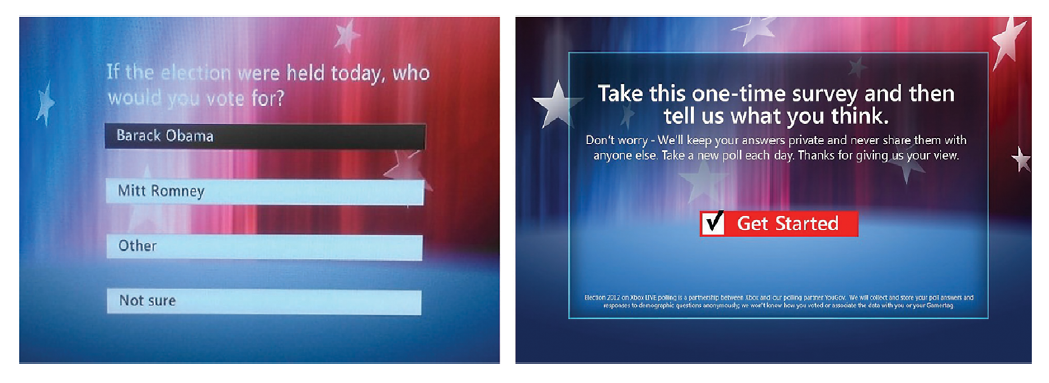
\includegraphics[width=\textwidth]{images/wangetal2}
\end{center}

{\footnotesize Wang et al. 2015. ``Forecasting elections with non-representative polls.'' \textit{International Journal of Forecasting}.\par}

}


\frame{
\frametitle{The Xbox Study}

\begin{center}
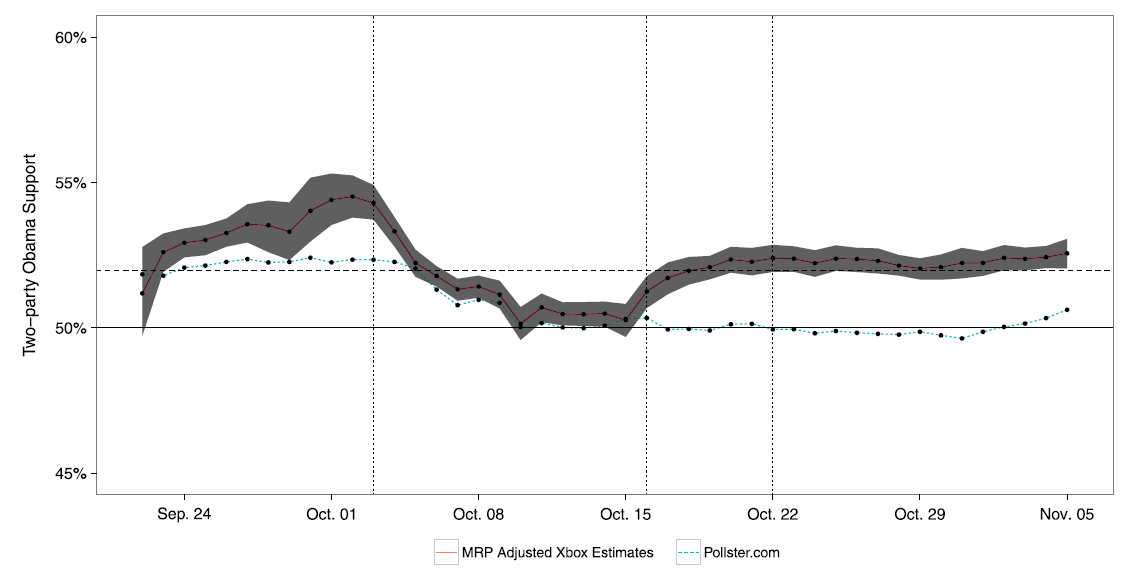
\includegraphics[width=\textwidth]{images/wangetal1}
\end{center}

\vspace{1em}

{\footnotesize Wang et al. 2015. ``Forecasting elections with non-representative polls.'' \textit{International Journal of Forecasting}.\par}

}



\frame{
\begin{center}
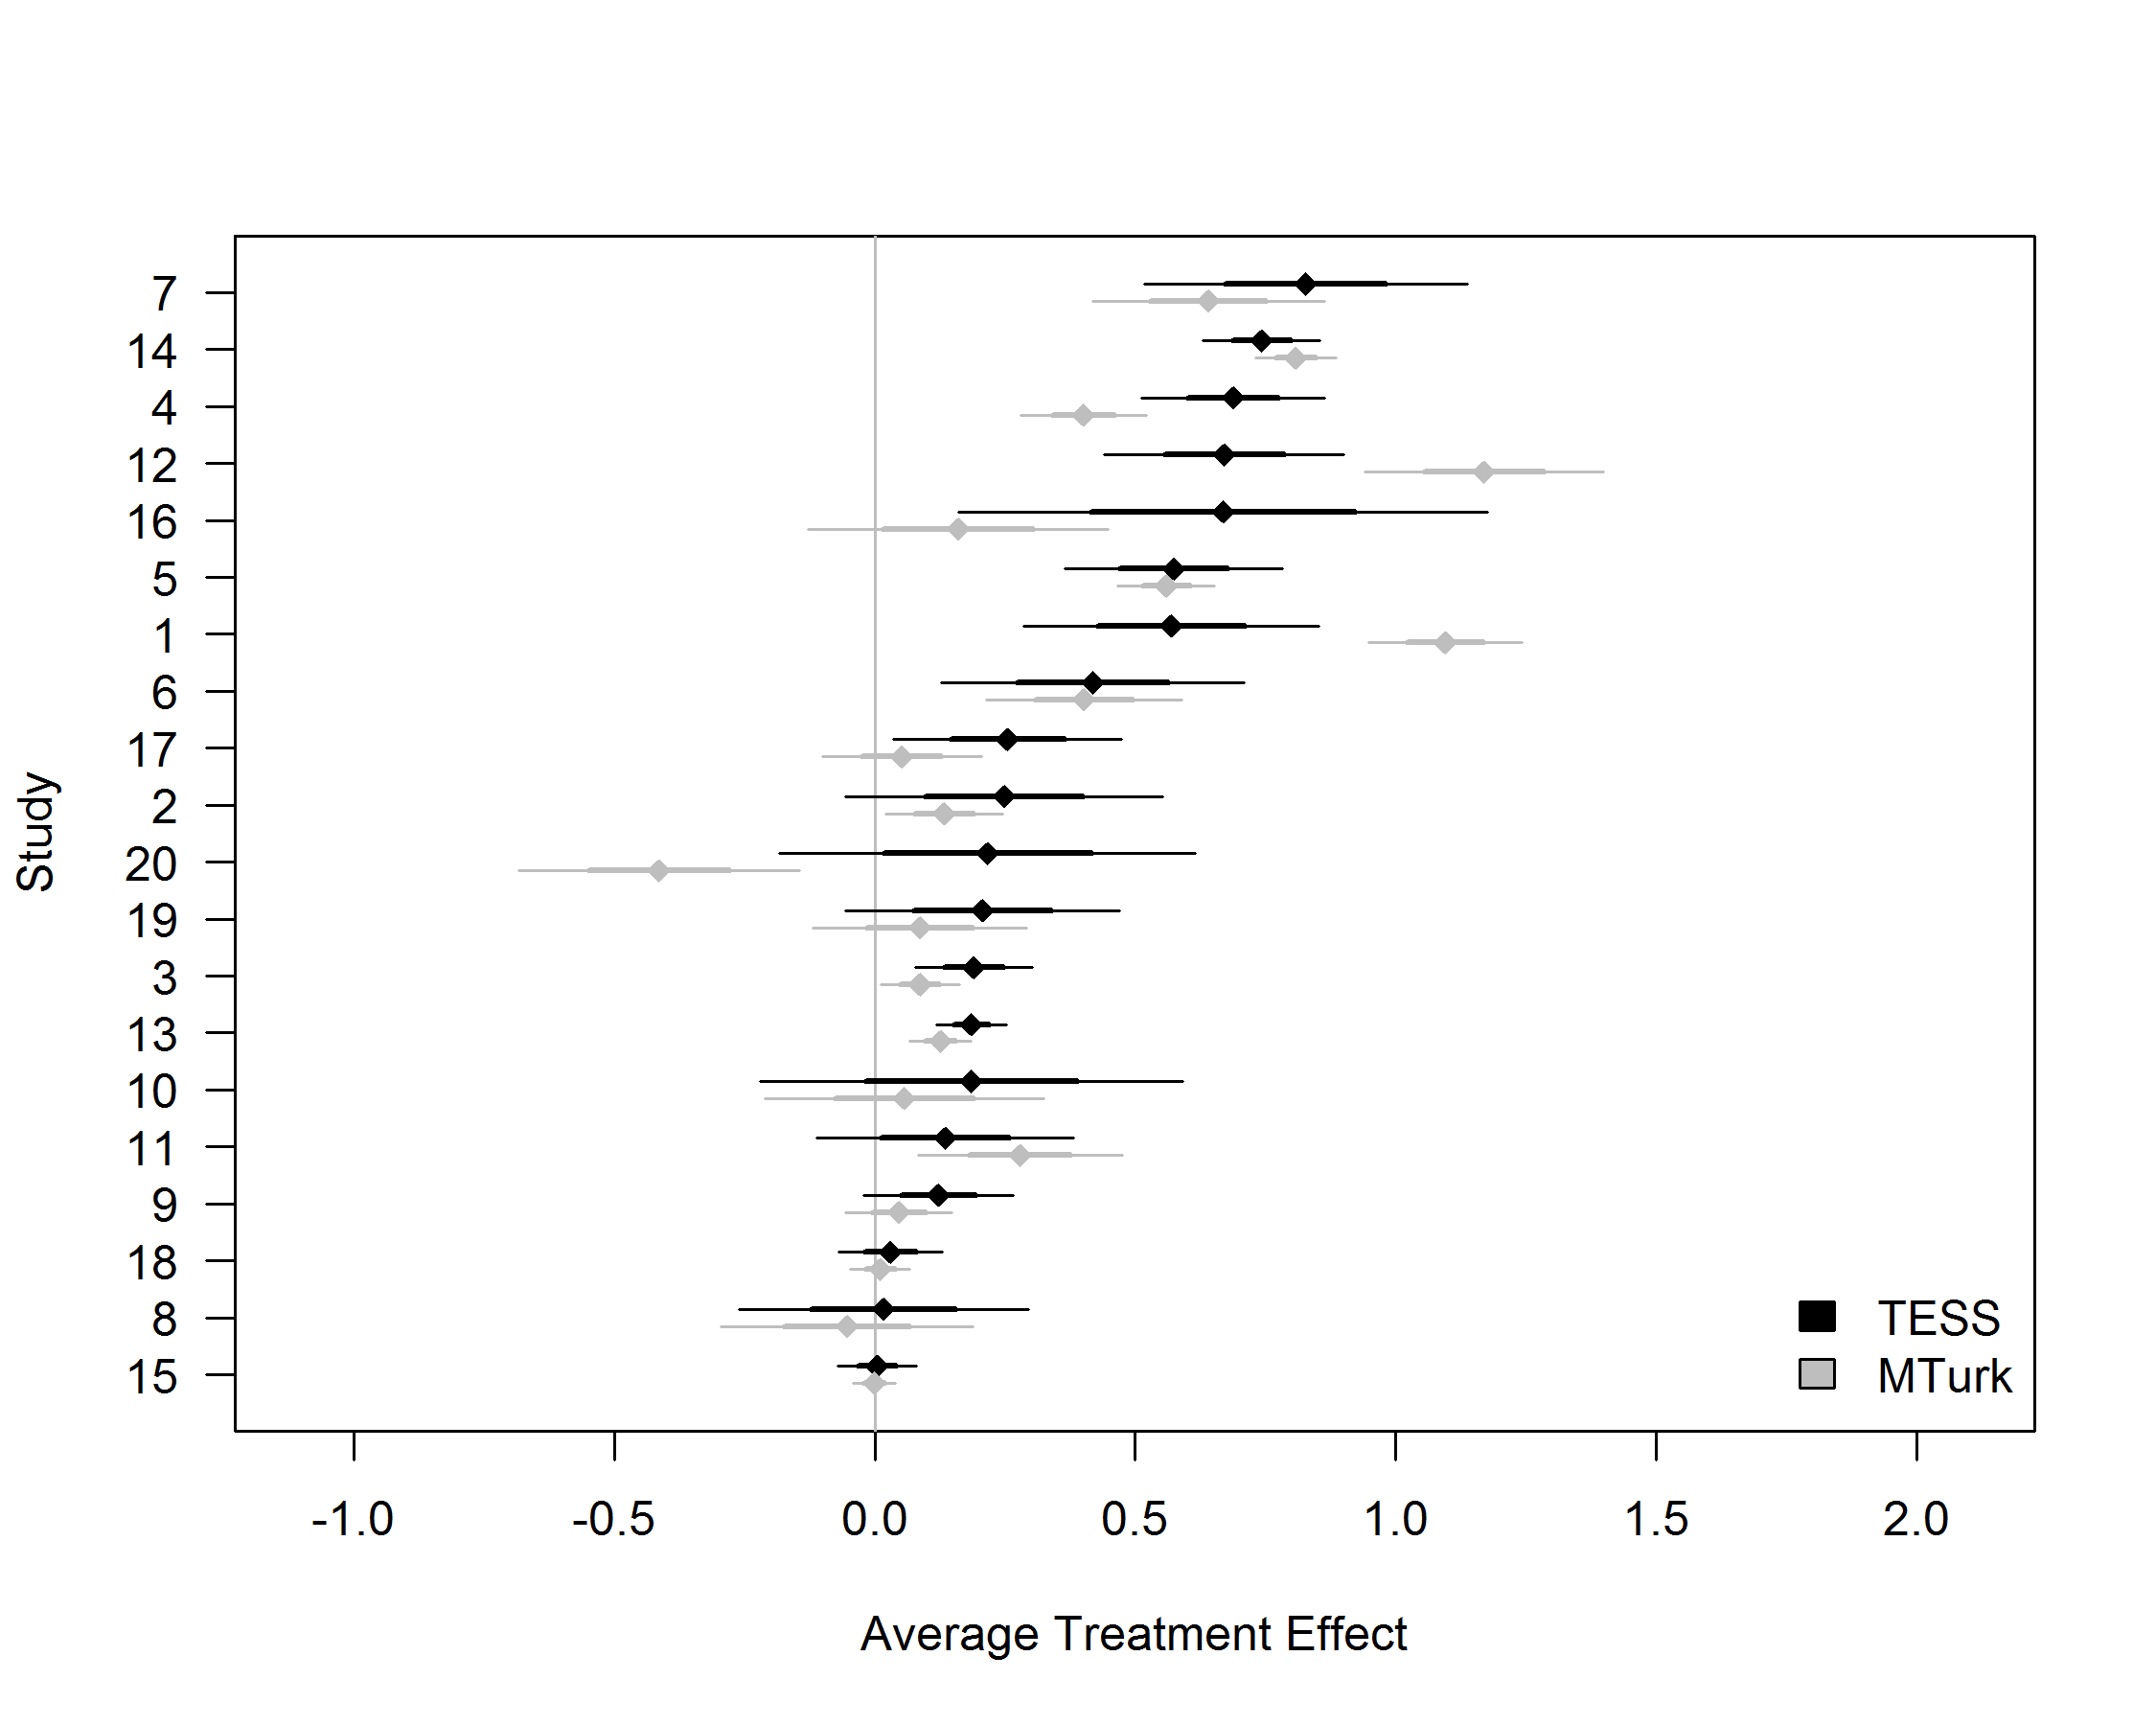
\includegraphics[width=.85\textwidth]{images/mullinix1}
\end{center}
\vspace{0.5em}
{\footnotesize Mullinix et al. In press. ``The Generalizability of Survey Experiments.'' \textit{Journal of Experimental Political Science}.\par}
}

\frame{
\begin{center}
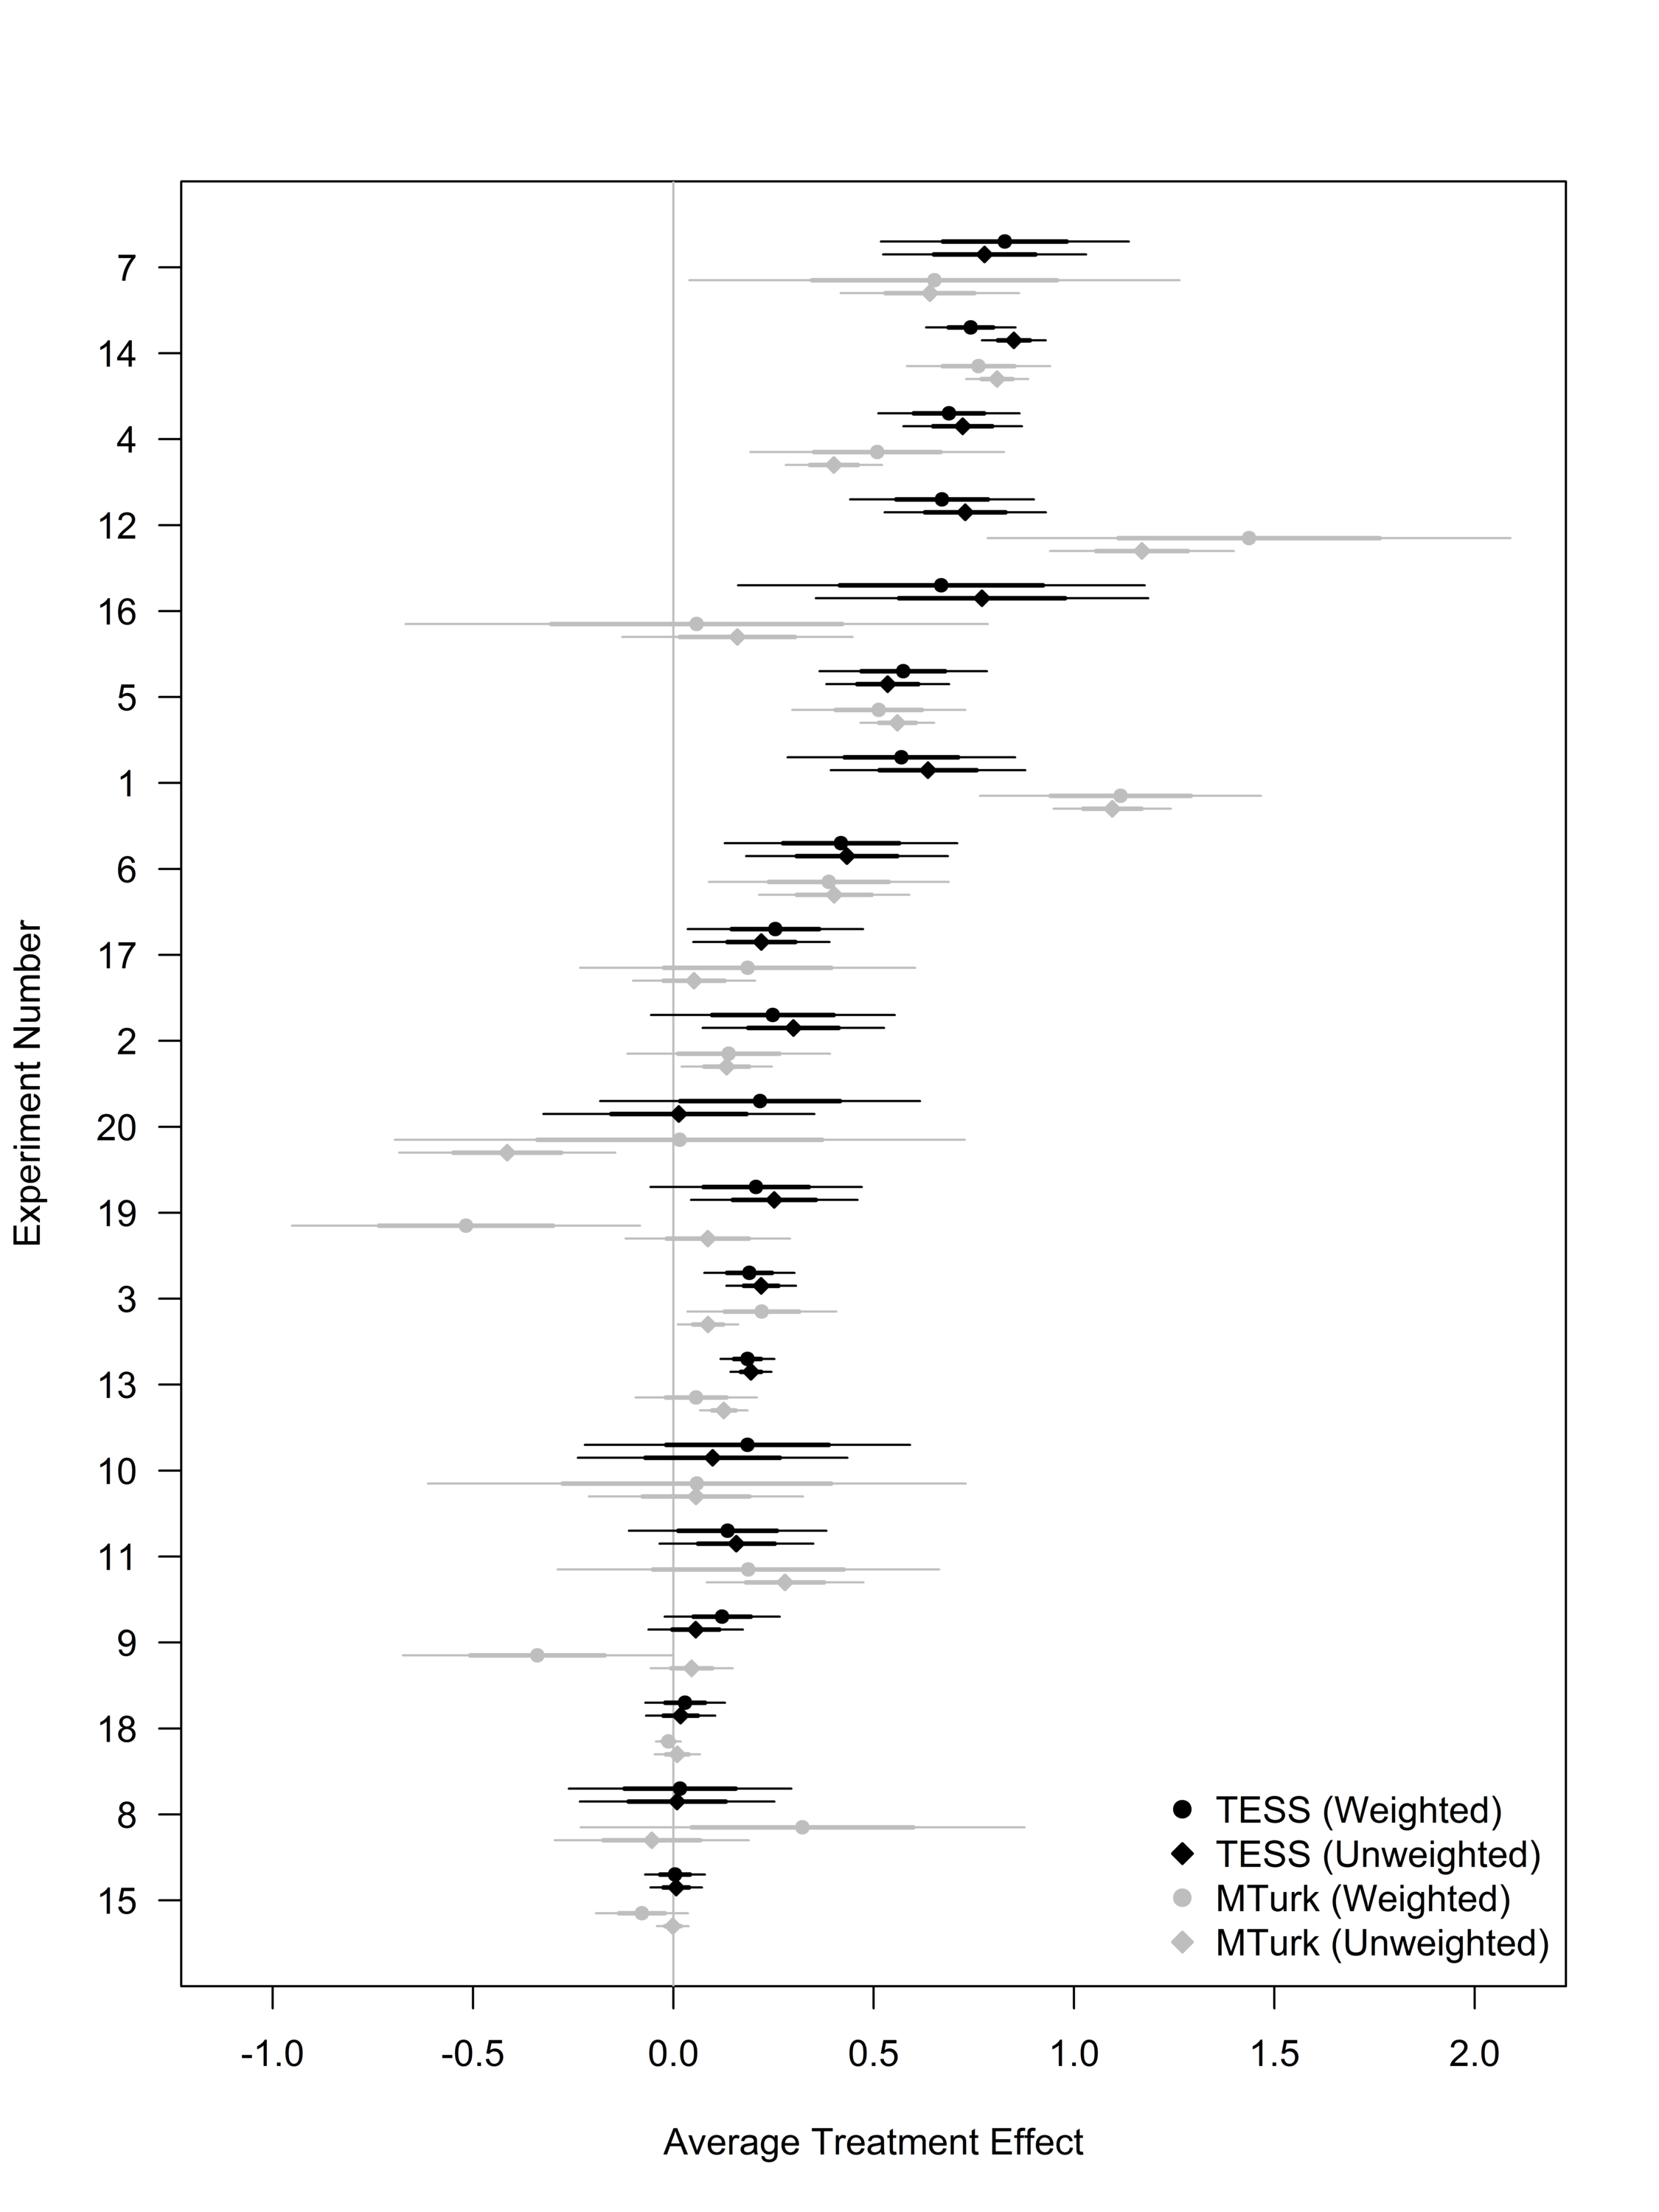
\includegraphics[width=.8\textheight]{images/mullinix2}
\end{center}
}



\frame{
\frametitle{Propensity Score Approach}
\begin{enumerate}
\item Define a target population to which sample inference is intended to generalize
\item Estimate a propensity score model
	\begin{itemize}
	\item Pool experimental samples and target population units
	\item Predict membership of all target and sample units in the experimental sample
	\end{itemize}
\item Using fitted logits, divide the population and sample into strata
	\begin{itemize}
	\item Number of strata is commonly 5 (Cochran, 1968)
	\end{itemize}
\item Estimate stratum-specific ATE
\item Calculate weighted average of stratum-level estimates
\end{enumerate}
}


\frame{
\frametitle{Propensity Score Approach}

Target population average treatment effect:
\begin{equation}
\sum_{v=1}^{5} p(v)T(v)
\end{equation}
where $p(v)$ is the proportion of the target population in a given stratum, $v$, and $T(v)$ is the estimated effect from stratum $v$ of the experimental sample
}


\frame{
\frametitle{Propensity Score Approach}

Effect variance:
\begin{equation}
\sum_{v=1}^{5} p(v)^2 V(v),
\end{equation}
where $V(v)$ is the variance of the estimated experimental sample effect for stratum $v$
}



\frame{
\frametitle{Propensity Score Subclassification Estimator}
\begin{columns}
\column{\dimexpr\paperwidth-15pt}
\scriptsize
\begin{tabular}{rrrrrrrrr} \toprule
& \multicolumn{2}{c}{Weights} & \multicolumn{6}{c}{Estimates}\\
Stratum & Nat'l & Sample & Loan & DREAM (Pro) & DREAM (Con) & Rally (All) \\% & Rally (Distant) & Rally (Local) \\ 
  \midrule
  1 & 0.20 & 0.83 & 0.94 (0.08) & 0.06 (0.11) & -0.22 (0.12) & 0.74 (0.10) \\% & 0.77 (0.15) & 0.72 (0.15) \\ 
  2 & 0.20 & 0.11 & 0.99 (0.26) & 0.22 (0.37) & -0.28 (0.36) & 0.77 (0.29) \\% & 0.85 (0.39) & 0.70 (0.42) \\ 
  3 & 0.20 & 0.04 & 1.28 (0.43) & -0.61 (0.58) & -1.76 (0.54) & 1.00 (0.45) \\% & 0.75 (0.64) & 1.26 (0.64) \\ 
  4 & 0.20 & 0.01 & 1.99 (0.73) & 0.29 (1.12) & 0.56 (0.89) & 1.44 (0.79) \\% & 3.13 (1.95) & 1.54 (0.63) \\ 
  5 & 0.20 & 0.00 &  &  &  &  &  &  \\ \midrule
  Sample & - & - & 1.04 (0.30) & -0.01 (0.44) & -0.34 (0.38) & 0.79 (0.33) \\% & 1.05 (0.60) & 0.86 (0.37) \\ 
  Nat'l & - & - & 1.14 (0.18) & 0.02 (0.22) & -0.94 (0.23) & 0.94 (0.19) \\% & 1.01 (0.26) & 0.93 (0.27) \\ 
   \bottomrule
\end{tabular}
\end{columns}
}


\frame{
\textbf{So does reweighting solve everything forever?}

\begin{itemize}\itemsep1em
\item<2-> Need well-defined target population
	\begin{itemize}
	\item and detailed covariate data
	\item and large stratum sizes
	\end{itemize}
\item<3-> Purely model-based, so only as good as the model
	\begin{itemize}
	\item What unobservables might be hiding bias?
	\item What reweighting might worse bias?
	\end{itemize}
\item<4-> Non-coverage is a potentially huge problem
\item<5-> Not well-tested on experimental data
\end{itemize}

}







% mode effects
\frame{
\frametitle{Mode Effects and Comparisons}
\begin{itemize}\itemsep1em
\item Behavioral research is historically lab-based
\item<2-> Online mode is different in many ways aside from \textit{mode}
	\begin{itemize}
	\item Self-paced
	\item Anonymous
	\item Private
	\item Computer-based
	\item General loss of experimental control
	\end{itemize}
\item<3-> Two big consequences
	\begin{itemize}
	\item Attrition
	\item Lower attention
	\end{itemize}
\end{itemize}
}


% attrition
\frame{
\frametitle{Attrition}
\begin{itemize}\itemsep1em
\item We care about two issues:
	\begin{itemize}
	\item Who leaves a study early
	\item When they leave a study
	\end{itemize}
\item<2-> We care about representativeness (not just demographically)
\item<3-> Analyze when participants leave study to identify difficult, confusing, or problematic study elements
	\begin{itemize}
	\item Ideally, do pilot tests
	\end{itemize}
\end{itemize}

}

% custom panels (from MTurk or elsewhere)
\frame{
\frametitle{Custom Panels}
\begin{itemize}\itemsep1em
\item Creating your own panel is great
	\begin{itemize}
	\item Carefully sample on specific characteristics % stanford model; qualification model; database model
	\item Organize repeated interviewing or interaction
	\end{itemize}
\item Lots of additional issues
	\begin{itemize}
	\item Attrition
	\item Compensation
	\item Panel Conditioning
	\end{itemize}
\item See Callegaro et al. 2014. \textit{Online Panel Research: A Data Quality Perspective}. Wiley.
\end{itemize}
}





% attention checks
\frame{
\frametitle{Attention Checking}

\large 
\begin{itemize}\itemsep1em
\item Online mode invites satisficing
\item Attention checking can help, but is imperfect
\end{itemize}
}

% useful for checking attention
% may have consequences for representativeness and introduce selection biases

\frame{
\frametitle{Apparent Satisficing}
\begin{itemize}\itemsep0.5em
\item Filter out respondents based on response behavior
\item Some common measures:
	\begin{itemize}
	\item ``Straightlining''
	\item Non-differentiation
	\item Acquiescence
	\item Nonresponse
	\item DK responding
	\item Speeding
	\end{itemize}
\item Difficult to detect
\item Difficult to distinguish from ``real'' responses
\end{itemize}
}

\frame{
\frametitle{Metadata/Paradata}
\begin{itemize}\itemsep1em
\item<1-> Timing
	\begin{itemize}
	\item Some survey tools will allow you to time page
	\item Make a prior rules about dropping participants for speeding
	\end{itemize}
\item<2-> Mousetracking or eyetracking
	\begin{itemize}
	\item Mousetracking is unobtrusive
	\item Eyetracking requires participants opt-in
	\end{itemize}
\item<3-> Record focus/blur browser events
\end{itemize}
}

\frame{
\frametitle{Direct Measures}
\begin{itemize}\itemsep2em
\item How closely have you been paying attention to what the questions on this survey actually mean?
\item<2-> While taking this survey, did you engage in any of the following behaviors? Please check all that apply.
	\begin{itemize}
	\item Use your mobile phone
	\item Browse the internet
	\item \dots
	\end{itemize}
\end{itemize}
}


\frame{
\frametitle{Substantive Manipulation Check}
\begin{itemize}\itemsep1em
\item Two common approaches:
	\begin{itemize}
	\item Information recall or understanding
	\item Measure level of manipulated treatment variable
	\end{itemize}
\item Risky to remove cases based on this because it is a form of conditioning on post-treatment variables
\item May be useful to consider either a mediator of effects
\end{itemize}
}

\frame{
\frametitle{Instructional Manipulation Check}

\only<2>{Do you agree or disagree with the decision to send British forces to fight ISIL in Syria? }We would like to know if you are reading the questions on this survey. If you are reading carefully, please ignore this question, do not select any answer below, and click ``next'' to proceed with the survey.\\

\vspace{1em}

\small

Strongly disagree\\
Somewhat disagree\\
Neither agree nor disagree\\
Somewhat agree\\
Strongly agree\\

}


\frame{
\frametitle{Attention Checking}

In summary\dots

\begin{itemize}\itemsep1em
\item Attention checking can be useful
\item Lots of options
\item No obvious best metric
\item Can be analytically consequential
\end{itemize}
}



\frame{}


\frame{
\frametitle{To Sum Up\dots}

\begin{itemize}\itemsep1em
\item Nationally representative samples are a hypothetical gold standard for behavioral research
\item We can get a lot of leverage from non-representative samples
\item Online context also enables innovative designs
\item Wide array of tools available to implement experiments and recruit participants
\end{itemize}
}


\frame{

\frametitle{Thanks!}

I will be around for questions.\\

\vspace{1em}

But don't hesitate to be in touch later on:\\

\begin{itemize}\itemsep0.5em
\item Slides: \url{http://www.thomasleeper.com/websurveycourse}
\item Email: \href{mailto:thosjleeper@gmail.com}{thosjleeper@gmail.com}
\item Twitter: \href{https://twitter.com/thosjleeper}{@thosjleeper}
\item GitHub: \href{https://github.com/leeper}{@leeper}
\end{itemize}


}




\appendix
\frame{}

\section{References}

\frame{
\frametitle{Experimental Methods}
\begin{itemize}\itemsep1em
\item Druckman et al. 2011. \textit{Cambridge Handbook of Experimental Political Science}. Cambridge.
\item Gerber and Green. 2011. \textit{Field Experiments}. W.W. Norton.
\item Mutz. 2011. \textit{Population-Based Survey Experiments}. Princeton.
\item Shadish et al. 2001. \textit{Experimental and Quasi-Experimental Designs for Generalized Causal Inference}. Houghton Mifflin.
\end{itemize}
}

\frame{
\frametitle{Survey Methods}
\begin{itemize}\itemsep1em
\item Groves et al. 2008. \textit{Survey Methodology}. 2nd Edition. Wiley.
\item Lohr. 2010. \textit{Sampling: Design and Analysis}. 2nd Edition. Cengage.
\end{itemize}
}


\frame{
\frametitle{Online Surveys}
\begin{itemize}\itemsep1em
\item Callegaro et al. 2015. \textit{Web Survey Methodology}. Sage.
\item Callegaro et al. 2015. \textit{Online Panel Research: A Data Quality Perspective}. Wiley.
\end{itemize}
}

\end{document}
